\documentclass[11pt,a4paper,oneside]{report}

\usepackage{amsmath,amssymb}
\usepackage{parskip}
\usepackage{graphicx}
\usepackage{xcolor}
\usepackage[a4paper,margin=1in]{geometry}
\usepackage{longtable,booktabs,array}
\usepackage{float}
\usepackage{algorithm}
\usepackage{algorithmic}
\usepackage{tikz}
\usepackage{amssymb}

\usetikzlibrary{shapes.geometric, arrows}

\usepackage{titlesec}
\titleformat{\chapter}[display]
  {\sffamily\bfseries\huge}
  {\Large \chaptertitlename\ \thechapter}
  {2ex}
  {\titlerule
  \vspace{1ex}%
  \filright\MakeUppercase}
  [\vspace{1ex}%
\titlerule]
\titleformat{\section} {\normalfont\sffamily\Large\bfseries} {\thesection}{1em}{}
\titleformat{\subsection} {\normalfont\sffamily\large\bfseries} {\thesubsection}{1em}{}
\titleformat{\subsubsection} {\normalfont\sffamily\normalsize\bfseries} {\thesubsubsection}{1em}{}
\usepackage[backend=biber, style=numeric-comp, sorting=none]{biblatex}
\addbibresource{bibfile.bib}

\usepackage[no-math]{fontspec}
\usepackage{unicode-math}
\defaultfontfeatures{Ligatures=TeX}
\setmainfont{Source Serif Pro}[BoldFont={Source Serif Pro Semibold}]
\setsansfont{SourceSansPro-Regular}[BoldFont={SourceSansPro-Semibold}]
\IfFontExistsTF{Cambria Math} {\setmathfont{Cambria Math}[Scale=1]} {\setmathfont{Asana Math}}

\usepackage{xeCJK}
\setCJKmainfont{Noto Sans SC}
\setCJKsansfont{Noto Sans SC}

\newcommand{\instructions}[1]{{\color{black}\itshape #1}}

\usepackage{upquote}
\usepackage[allcolors=blue,colorlinks=true]{hyperref}
\usepackage{xurl}
\usepackage{microtype}
\usepackage{bookmark}
\usepackage{calc}
\usepackage{etoolbox}

\usepackage{setspace}

\urlstyle{same}

\begin{document}

\onehalfspacing

% Author name (capitalized in its regular way)
\newcommand{\authorname}{Jingheng Huan}

% Title (cannot exceed three lines)
% You can insert manual linebreaks with \
\newcommand{\thetitle}{A CASE STUDY OF AI IN VISION AND SOUND GENERATION: THE EVOLUTION, APPLICATIONS, AND ETHICAL CONSIDERATIONS}

% Date of submission with normal capitalization. 
% Use the format January 29, 2022.
\newcommand{\submissiondate}{Mar 7, 2024}

% Mentor: First Name Last Name (normal capitalization)
\newcommand{\mentor}{Peng Sun}

% Academic Unit (no abbreviations)
\newcommand{\academicunit}{Division of Natural and Applied Sciences}

%%%%%%%%%%%%%%%%%%%%%%%%%%%%%%%%%%%%%%%%%%%%%%%%%%%%%%%%%%%%%%%%%%%%%%%%%%%%%%%%

%% DO NOT CHANGE DIRECTLY THE CONTENTS OF THE TITLE PAGE.
%% TO CUSTOMIZE THE TITLE PAGE CHANGE THE DEFINITIONS OF THE COMMANDS
%% \authorname, \thetitle, \submissiondate, \mentor, \academicunit


\begin{titlepage}

\vspace*{\bigskipamount}

\begin{center}
{\sffamily\LARGE\bfseries\MakeUppercase\thetitle\par}

\bigskip

by

\bigskip

{\Large \authorname}

\bigskip

Signature Work Product, in partial fulfillment of the \\
Duke Kunshan University Undergraduate Degree Program

\bigskip

\emph{\submissiondate}

\bigskip

Signature Work Program \\
Duke Kunshan University

\end{center}

\vfill

\textbf{\textsf{APPROVALS}}

\bigskip\bigskip\bigskip
\hrule

Mentor: \mentor, \academicunit

\bigskip\bigskip\bigskip
\hrule

Marcia B. France, Dean of Undergraduate Studies

\end{titlepage}

%%%%%%%%%%%%%%%%%%%%%%%%%%%%%%%%%%%%%%%%%%%%%%%%%%%%%%%%%%%%%%%%%%%%%%%%%%%%%%%%

% Front matter
\clearpage
\pagenumbering{roman}

%%%%%%%%%%%%%%%%%%%%%%%%%%%%%%%%%%%%%%%%%%%%%%%%%%%%%%%%%%%%%%%%%%%%%%%%%%%%%%%%

\setcounter{tocdepth}{1} % Only top-level units (chapters) should appear in the TOC
\tableofcontents

%%%%%%%%%%%%%%%%%%%%%%%%%%%%%%%%%%%%%%%%%%%%%%%%%%%%%%%%%%%%%%%%%%%%%%%%%%%%%%%%

\chapter*{Abstract}
\addcontentsline{toc}{chapter}{Abstract}

% Abstract in English

\instructions{This study embarks on an in-depth exploration of the transformative impact of Artificial Intelligence (AI) on the realms of image, video, and sound generation. It presents a comparative analysis of cutting-edge AI technologies, including Generative Adversarial Networks (GANs), Diffusion Models, and Neural Cellular Automata, highlighting their development, theoretical underpinnings, and practical applications. The research delves into the significant advancements these technologies have made possible, showcasing their ability to produce highly realistic and creative outputs. Moreover, it addresses the crucial ethical considerations surrounding the use of AI in content creation, emphasizing the need for robust guidelines to ensure the responsible deployment of these technologies. The findings of this study underline the potential of AI to revolutionize digital media production, pushing the boundaries of creativity and opening up new possibilities for innovation across various sectors. This abstract provides a concise overview of the research's scope, methodologies, and key contributions, setting the stage for a deeper discussion on the evolving role of AI in shaping the future of digital media.}

\vspace{4\bigskipamount}

% Abstract in Chinese

\paragraph{\textnormal{本研究深入探讨了人工智能(AI)在图像、视频和声音生成领域的变革性影响。通过对最先进的AI技术进行比较分析,包括生成对抗网络(GANs)、扩散模型和神经细胞自动机,突出展示了这些技术的发展、理论基础和实际应用。研究深入探讨了这些技术实现的重大进步,展示了它们产生高度逼真和富有创造性输出的能力。此外,它还讨论了AI在内容创作中使用的关键伦理考虑,强调需要制定严格的指导方针,以确保这些技术的负责任部署。本研究的发现强调了AI革新数字媒体生产的潜力,推动创造力的边界,并在各个领域开辟了创新的新可能性。这个摘要提供了对研究范围、方法论和主要贡献的简洁概述,为深入讨论AI在塑造数字媒体未来中的不断发展作用奠定了基础。}}

%%%%%%%%%%%%%%%%%%%%%%%%%%%%%%%%%%%%%%%%%%%%%%%%%%%%%%%%%%%%%%%%%%%%%%%%%%%%%%%%

\chapter*{Acknowledgements}
\label{acknowledgements}
\addcontentsline{toc}{chapter}{Acknowledgements}

\instructions{I would like to express my sincere gratitude to my SW mentor, Prof. Peng Sun, 
for his invaluable guidance throughout this research. 
Also, I am grateful to the other members of the SW team for their support and guidance. 
In the end, I would like to thank the SW office for their support and guidance, 
and also extend my thanks to the generous funding provided by SW grants, ¥1800, which made the experiential learning part possible. 
Finally, I would like to thank my family and friends for their support and encouragement. 
}

\newpage

%%%%%%%%%%%%%%%%%%%%%%%%%%%%%%%%%%%%%%%%%%%%%%%%%%%%%%%%%%%%%%%%%%%%%%%%%%%%%%%%

% Add captions to your figures for them to appear in the List of Figures.
% Alternatively, comment out the next two lines if there are no tables 
% in your document.
\addcontentsline{toc}{chapter}{List of Figures}
\setcounter{tocdepth}{1}
\listoffigures\newpage

%%%%%%%%%%%%%%%%%%%%%%%%%%%%%%%%%%%%%%%%%%%%%%%%%%%%%%%%%%%%%%%%%%%%%%%%%%%%%%%%

% Add captions to your tables for them to appear in the List of Tables.
% Alternatively, comment out the next two lines if there are no tables 
% in your document.
%%%%%%%%%%%%%%%%%%%%%%%%%%%%%%%%%%%%%%%%%%%%%%%%%%%%%%%%%%%%%%%%%%%%%%%%%%%%%%%%

% Main matter

\clearpage
\pagenumbering{arabic}

%%%%%%%%%%%%%%%%%%%%%%%%%%%%%%%%%%%%%%%%%%%%%%%%%%%%%%%%%%%%%%%%%%%%%%%%%%%%%%%%

\chapter{Introduction}
\label{introduction}

\section{Artificial Intelligence (AI)}
Artificial Intelligence (AI) is an expansive field that integrates principles from computer science, mathematics, and neuroscience to set up systems capable of simulating human cognitive functions and executing tasks traditionally requiring human intellect \cite{russell2010artificial}. 
This interdisciplinary approach transforms AI from a mere conceptual framework into an indispensable tool across diverse sectors such as technology, finance, and entertainment. 
The core of AI's functionality is its ability to learn from data and make decisions autonomously, without hard coding the explicit instructions. 
One of the foundational models in AI's evolution is machine learning \cite{jordan2015machine}, which includes techniques for classification, regression, and clustering \cite{huang2022large}. 
These methods allow computers to learn patterns and make predictions from data, forming the basis for many early AI applications. 
As the field matured, researchers developed more sophisticated models, including neural networks \cite{abiodun2018state}, which imitate the structure and function of the human brain to perform complex pattern recognition tasks \cite{schmidhuber2015deep}.

The evolution of AI is marked by significant milestones, particularly with the advent of deep learning \cite{lecun2015deep} techniques, which have revolutionized areas like computer vision \cite{voulodimos2018deep} and natural language processing (NLP) \cite{chowdhary2020natural}. 
Deep learning, a subset of machine learning, employs complex neural networks with multiple layers of processing units, enabling the extraction of high-level features from raw input data. 
It improved the performance of AI systems in tasks ranging from image and speech recognition to language translation \cite{goodfellow2016deep}.
Recent years some specialized architectures have further pushed the boundaries of what AI can achieve. 
Variational Autoencoders (VAE), \cite{rezende2014stochastic, kingma2013auto}, Generative Adversarial Networks (GANs)~\cite{goodfellow2014generative, vondrick2016generating, tulyakov2018mocogan, clark2019adversarial, brooks2022generating}, and diffusion models \cite{rombach2022high, ho2022imagen, blattmann2023align, gupta2023photorealistic} represent the forefront of AI research in data generation. 
GANs consist of two neural networks—the generator and the discriminator—competing against each other to generate new, synthetic instances of data that are indistinguishable from real data. 
This has proven especially powerful in the fields of vision and sound generation, enabling the creation of photorealistic images, videos, and lifelike synthetic audio \cite{granot2022drop}.

The advancements in AI have not only expanded the horizons of what is technically feasible but have also paved the way for innovations in digital content creation that were previously unimaginable. 
The development and application of StyleGAN \cite{karras2019style} and its successors have been pivotal in pushing the limits of image generation technologies. 
These models have the remarkable ability to produce images of astonishing realism, manipulate facial expressions with precision, and even venture into the realm of digital art creation \cite{patashnik2021styleclip}. 
Similarly, the advent of diffusion models marks a significant leap in the quality of generated content, setting unprecedented standards for both image and sound generation \cite{rombach2022high}. 
These models operate by iteratively refining data inputs through a process that progressively reduces noise, allowing for the creation of outputs that are not only highly detailed but also deeply resonant with the nuances of real-world sensory experiences. 
Such advancements underscore the multifaceted impact of AI in the digital domain, where the synergy between complex neural networks and deep learning techniques is not just enhancing the visual and auditory quality of synthetic media but is also broadening the scope of creative expression and immersion in virtual environments. 
This ongoing evolution in AI-driven content generation reflects a convergence of insights from across computer science, mathematics, and neuroscience, highlighting the interdisciplinary effort that underpins AI's capability to reinterpret and reimagine the way machines understand and interact with the world around us \cite{silver2016mastering}.

\section{Artificial Intelligence Generated Content (AIGC)}

In the field of Artificial Intelligence Generated Content (AIGC), platforms like ChatGPT \cite{leiter2023chatgpt} \cite{openai2023gpt}, MidJourney \cite{MidjourneyExplore}, Runway \cite{runwayml}, and ElevenLabs \cite{elevenlabs} are redefining the boundaries of creative expression. 
ChatGPT, with its sophisticated large language model, excels in generating text that mocks human-like understanding and creativity, making it a helpful tool for crafting compelling narratives, dialogues, and even complex literary works. 
Its ability to process and produce coherent, contextually relevant content on a vast array of topics has democratized content creation, enabling writers and creators to generate high-quality text-based content efficiently. 
Similarly, MidJourney revolutionizes the visual aspect of content creation by transforming textual descriptions into detailed, high-resolution images, and also style transformation.
This AI-driven approach to art and design allows creators to visualize abstract concepts and bring their most imaginative ideas to life, significantly simplifying the visual image storytelling process. 
Runway offers a toolkit of video generation and editing powered by AI, enabling creators to automate labor-intensive tasks such as object detection, background removal, and even generating video clips from textual prompts. 
This not only streamlines the video production process but also opens up new avenues for creativity and experimentation in visual content. 
ElevenLabs, with its state-of-the-art voice synthesis technology, provides solutions for text to speech and speech to text, changing the language of a speech, and even cloning the voice.
Whether for dubbing, voiceovers, or virtual assistants, ElevenLabs offers unparalleled customization, allowing for the creation of unique vocal identities that can speak in multiple languages and tones. 
The combination of these AI models—ChatGPT, MidJourney, Runway, and ElevenLabs prelude a new age in digital content creation, where the fusion of text, image, video, and voice generated through AI not only enriches the content landscape but also offers creators the tools to craft experiences that were once unimaginable.

However, AIGC technology has also sparked ethical debates concerning the creation and use of AI-generated content. 
Deepfakes \cite{westerlund2019emergence}, which involve altering videos and images to the point of being indistinguishable from authentic media, have the potential to distort reality and spread misinformation. 
The manipulation of media content raises concerns about the impact on individuals' reputations and the broader implications for societal and political discourse. 
As artificial intelligence capabilities grow, the need for ethical guidelines that ensure transparency and prevent biases becomes more urgent.
Coupled with the ethical concerns surrounding deepfakes is the issue of copyright in AI-generated images and videos. \cite{hristov2016artificial}
The legal system is currently unprepared to tackle questions of ownership and violation when content is created by an AI. 
This prompts a discussion about the originality of AI-generated works and the ethical use of AI in creative processes. 
As AI becomes more pervasive, it will challenge traditional copyright laws, necessitating continuous research and the development of legal measures that keep pace with AI evolution.


\section{Current Development Trends}

The evolution of generative AI has unfolded with unexpected speed.
The transition from large, centralized systems to more accessible and powerful technologies has seen generative AI quickly reach a phase where enthusiasts and professionals can experiment and innovate with considerable autonomy. 
The proliferation of smaller, more efficient foundation models, such as Meta's LLaMa family \cite{touvron2023llama}, StableLM \cite{StabilityAI_StableLM}, and Mistral \cite{jiang2023mistral}, indicate a move towards greater performance with reduced resource requirements. 
These applications, alongside the increasing availability of open-source models, are democratizing AI by enabling a wider array of users to access state-of-the-art capabilities, fostering a more inclusive AI ecosystem.

\begin{figure}[htbp]
  \centering
  \includegraphics[width=0.9\textwidth]{timeline.png}
  \caption{A comprehensive overview of key milestones and product launches in the generative AI video domain throughout the year 2023, with a notable concentration of developments occurring in the fourth quarter. \cite{a16zAI2023}}
\end{figure}

As the demand for AI capabilities continues to surge, the AI industry faces practical challenges such as GPU shortages and rising cloud costs. 
This situation is pushing developers to innovate with hardware-efficient models and explore new deployment environments.
The ability to run smaller models locally on devices is particularly significant, offering privacy advantages and opening up possibilities for edge computing and IoT applications. 
The ability to customize and fine-tune AI models is becoming increasingly important for businesses looking to differentiate their services. 
Open-source models offer the flexibility to develop tailored AI solutions, trained on proprietary data and optimized for specific industry needs. 
This approach is particularly relevant in sectors like healthcare, legal, and finance, which require specialized knowledge and expertise to generate high-quality content.

\begin{figure}[htbp]
  \centering
  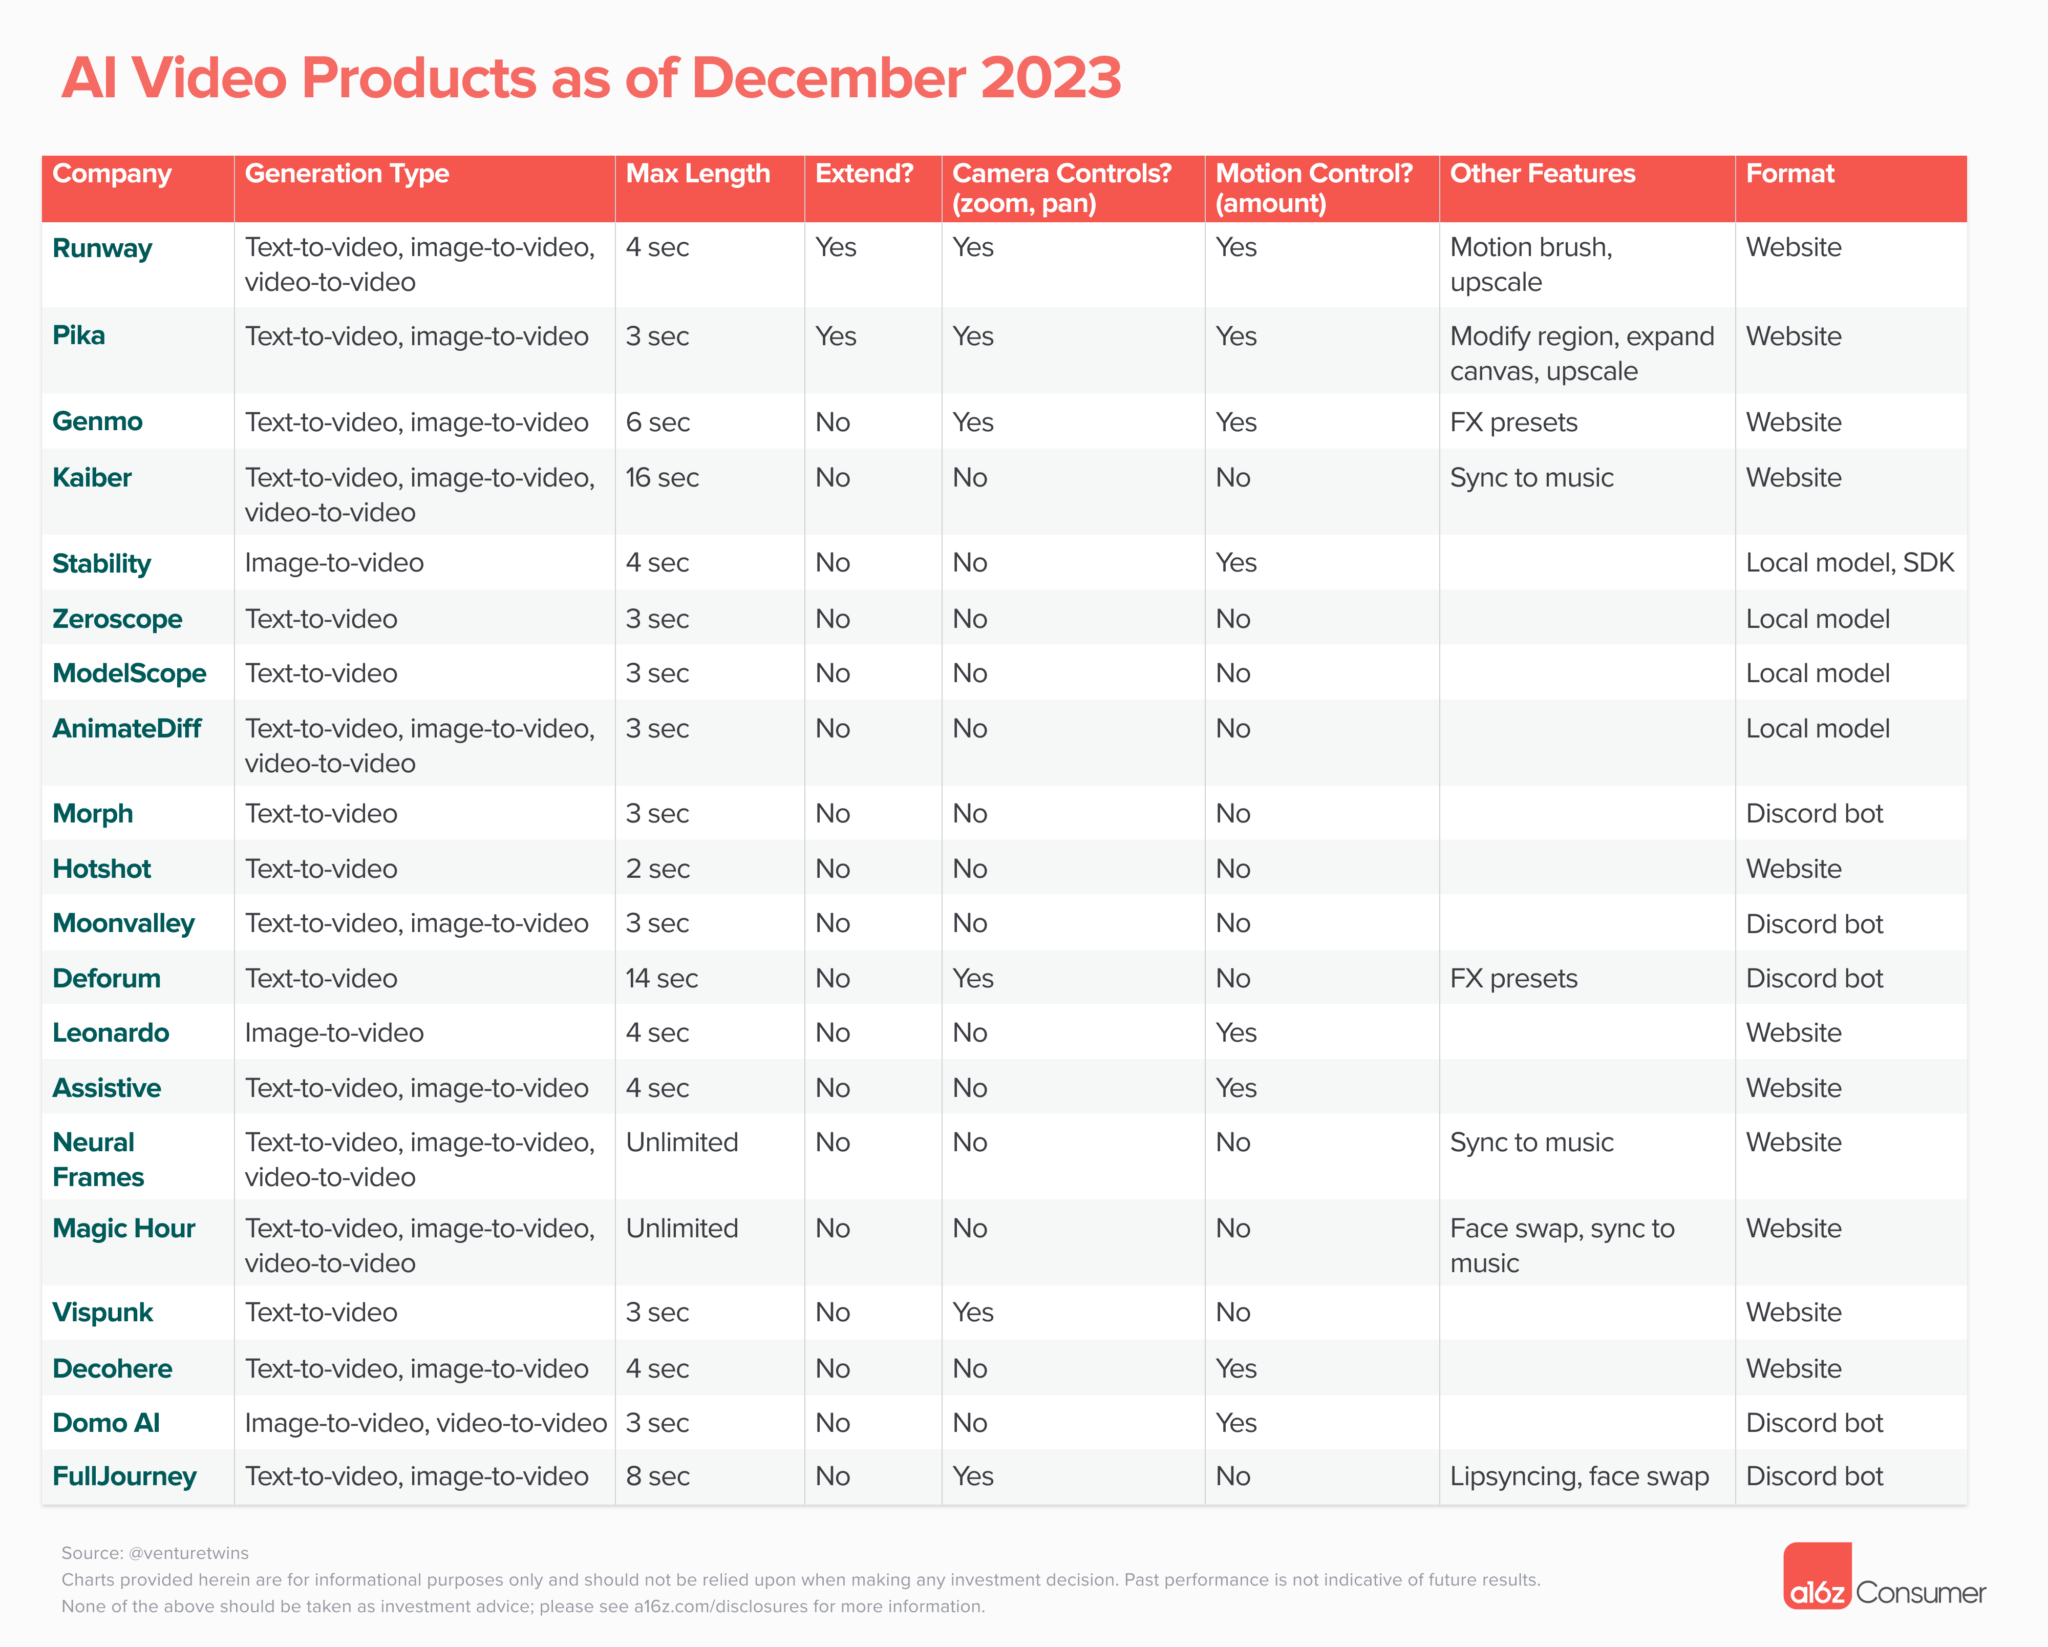
\includegraphics[width=0.9\textwidth]{products.png}
  \caption{Comparative analysis of various AI video product offerings as of December 2023, detailing generation types, maximum length of generated clips, and additional features such as camera and motion control, showcasing the diversity and capabilities within the current market landscape.\cite{a16zAI2023}}
\end{figure}

The regulatory environment for AI is rapidly evolving, with significant developments in the EU, China, and the US. 
The EU's provisional agreement on the AI Act \cite{eu_ai_act_2023}, China's measures to regulate AI usage \cite{China_AI_Policy_2023}, and the US's executive order on AI governance \cite{WhiteHouse_AI_ExecOrder_2023} reflect a global movement towards establishing legal frameworks to ensure responsible AI development and deployment. 
The outcome of ongoing legal battles, such as the New York Times' lawsuit against OpenAI \cite{Grynbaum_Mac_2023_Times_Sues_OpenAI}, may have far-reaching implications for the future of AI regulation and its impact on innovation and deployment. 
As we look towards the future, the most impactful developments in AI may well be centered around governance, middleware, and data pipelines that make generative AI more trustworthy and accessible. 
With a more refined understanding of AI capabilities, businesses are now focusing on integrating AI tools into existing services to enhance rather than revolutionize established processes. 
The challenge lies in striking a balance between leveraging the unique opportunities presented by AI while managing realistic expectations about its role in reshaping business practices.

\begin{figure}[htbp]
  \centering
  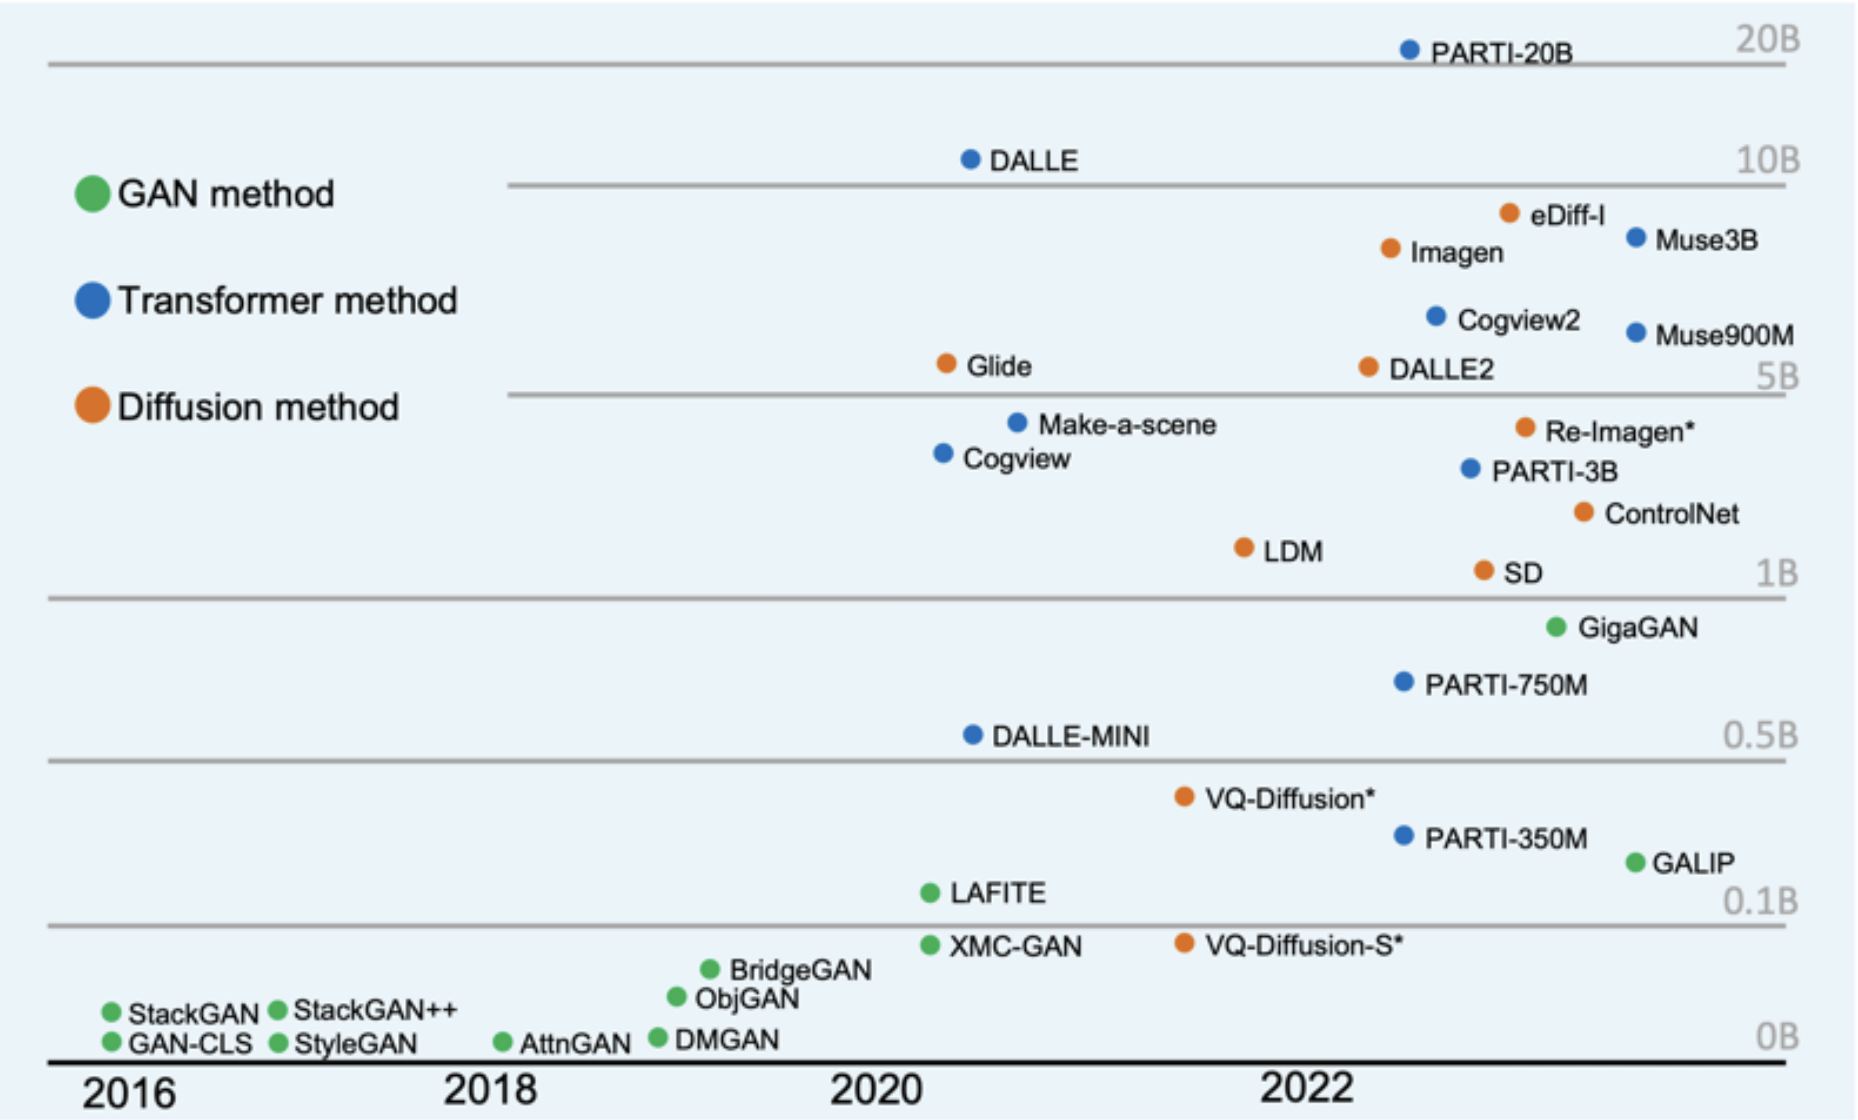
\includegraphics[width=0.9\textwidth]{models.png}
  \caption{Progression of generative modeling techniques from 2016 to 2022, showcasing the evolution and scaling of model parameters in GAN, Transformer, and Diffusion methods, each color-coded by method type.\cite{bie2023renaissance}}
\end{figure}

In the field of image generation, models like MidJourney, DALL-E 3, and Stable Diffusion 3 have been at the forefront. 
Video generation has also seen substantial growth, with platforms such as Runway Gen-2, Pika, and Sora pushing the boundaries of what can be achieved in AI-generated cinematography. 
In the audio domain, AI's capability to replicate and generate human-like speech has made significant strides with models such as ElevenLabs, Speechify, and Whisper. 
These tools have not only democratized voice-over and audio content production but have also raised the bar for what can be expected from synthetic speech in terms of clarity, emotion, and expressiveness. 
The geographical landscape of AI development is also noteworthy, with the United States and China emerging as the primary incubators of AI innovation. 
Leading internet companies in these countries, including tech giants like Google, Meta, Alibaba, and ByteDance, have been instrumental in driving forward the development of AI technologies. 
Their investments have resulted in state-of-the-art models that, while most of them are not open-source.

\chapter{Related Work}

\section{AIGC in Image and Video}

\subsection{Variational Autoencoders (VAE)}

Variational Autoencoders (VAEs) are a subclass of autoencoders that are foundational for generative models. They are composed of an encoder and a decoder \cite{cho2014properties}. The encoder transforms input data into a latent space, whereas the decoder reconstructs the input data from this space. The latent space is typically modeled as a Gaussian distribution, with the encoder providing the parameters—mean $\mu$ and variance $\sigma^2$—for this distribution.

The encoder part of a VAE is responsible for compressing the input data into a latent representation. For a given data element $x_i$, the encoder produces a mean $\mu_i$ and a variance $\sigma^2_i$ that define a Gaussian distribution in the latent space. The encoding process can be represented by the following equation:
\begin{equation}
\log q_{\phi} \left( z^{(i)} | x^{(i)} \right) = \log \mathcal{N} \left( z^{(i)}; \mu^{(i)}, \sigma^{2(i)} I \right).
\end{equation}

To allow for gradient descent methods to work, VAEs employ a reparameterization trick. This trick involves sampling a noise vector $\epsilon$ from a standard Gaussian distribution and then constructing the latent vector $z_i$ by scaling the noise with the standard deviation and shifting by the mean:
\begin{equation}
z_i = \mu_i + \epsilon \times \sigma_i,
\end{equation}
where $\epsilon \sim \mathcal{N}(0, I)$.

The decoder's goal is to reconstruct the input data from the latent representation. It tries to generate data that is as close as possible to the original input by maximizing the likelihood of the data given the latent space representation.

The training of VAEs involves maximizing the evidence lower bound (ELBO) on the marginal likelihood of the observed data. The ELBO can be represented as follows:
\begin{equation}
\mathcal{L}_b = -D_{KL}(q(z|x)||p(z)) + \frac{1}{L} \sum_{i=1}^{L}(\log P(x|z)).
\end{equation}
Furthermore, the ELBO can be decomposed into two terms: the first being the Kullback-Leibler divergence between the encoder's distribution and the prior distribution of the latent variables, and the second term being the expected log-likelihood of the data given the latent variables. For a latent space with dimensionality $d$, and assuming a standard Gaussian prior, the loss function simplifies to:
\begin{equation}
\mathcal{L}(\theta, x^i) = -\frac{1}{2} \sum_{i=1}^{d} \left( \mu^{2}_{(i)} + \sigma^{2}_{(i)} - \log \sigma^{2}_{(i)} - 1 \right) + \frac{1}{L} \sum_{i=1}^{L} \left( \log P(x^{i} | z) \right).
\end{equation}

Despite their advantages for generative tasks, VAEs have limitations, particularly for image generation. Directly sampling from the Gaussian distribution often results in blurred images. Moreover, there is an information loss when projecting the data to a lower-dimensional latent space, which affects the quality of the reconstruction. However, VAEs find extensive applications in feature extraction and dimensionality reduction, and they can be particularly effective when combined with other generative models such as Generative Adversarial Networks (GANs) or diffusion models.

\subsection{Generative Adversarial Networks (GAN)}

Generative Adversarial Networks (GANs) represent a class of generative models that has significantly impacted the field of synthetic image generation. A GAN is composed of two distinct neural network models: a \textit{generator} ($G$) and a \textit{discriminator} ($D$). The generator attempts to produce data that is indistinguishable from genuine data, while the discriminator evaluates the authenticity of the data, distinguishing between actual and generated samples.

The objective function of a GAN is formulated as a min-max game between $G$ and $D$:
\begin{align}
\min_{G} \max_{D} V(D, G) = \mathbb{E}_{x\sim p_{data}(x)}[\log D(x)] + \mathbb{E}_{z\sim p_{z}(z)}[\log (1 - D(G(z)))],
\end{align}
where $p_{data}$ is the data distribution, $x$ represents real data, $z$ is a noise sample from distribution $p_z$, and $G(z)$ is the generated data.

During training, $D$ is optimized to maximize the probability of correctly classifying a sample as real or fake. Simultaneously, $G$ is optimized to minimize $\log(1 - D(G(z)))$. In practice, this is often achieved by alternating between the following gradient ascent step for $D$:
\begin{align}
\nabla_{\theta_d} \frac{1}{m} \sum_{i=1}^{m} \Big[ \log D(x^{(i)}) + \log (1 - D(G(z^{(i)}))) \Big],
\end{align}
and the gradient descent step for $G$:
\begin{align}
\nabla_{\theta_g} \frac{1}{m} \sum_{i=1}^{m} \log (1 - D(G(z^{(i)}))),
\end{align}
for a minibatch of $m$ samples.

GANs have been utilized to generate high-fidelity images, outperforming other generative models in visual quality. However, they often struggle with mode collapse -- a phenomenon where the generator produces a limited variety of outputs. Despite these challenges, GANs have shown impressive results in tasks beyond image generation, such as image super-resolution \cite{denton2015deep}and object detection \cite{goodfellow2014generative}.

\subsection{Diffusion Models}

Diffusion models \cite{sohl2015deep, ho2020denoising} are a class of generative models famous for their ability to generate high-quality images through a process that iteratively adds and removes noise. These models are characterized by their use of a Markov chain to gradually convert simple noise distributions into complex data distributions.

A diffusion model typically consists of two main components: the forward process (described in Algorithm 1) and the reverse process (described in Algorithm 2). The forward process models the gradual addition of noise to the data, while the reverse process models the generation of data from noise. Mathematically, the forward process can be described by:
\begin{equation}
q(\mathbf{x}_t | \mathbf{x}_{t-1}) = \mathcal{N}(\mathbf{x}_t; \sqrt{1-\beta_t} \mathbf{x}_{t-1}, \beta_t \mathbf{I}),
\end{equation}
where $\beta_t$ is a variance schedule over discrete timesteps $t = 1, 2, ..., T$. 

\begin{algorithm}
\caption{Diffusion model training \cite{bie2023renaissance}}
\begin{algorithmic}[1]
\STATE for every training iteration do
\STATE \hspace{\algorithmicindent} Sample $t$ from discrete timestep $1, 2, \ldots, T$, or from continuous timestep $t \sim [0, 1]$.
\STATE \hspace{\algorithmicindent} Sample random noise $\epsilon \sim \mathcal{N}(0, 1)$.
\STATE \hspace{\algorithmicindent} Calculate $x_t$ based on DDPM forward or SDE forward.
\STATE \hspace{\algorithmicindent} Update the model with noise prediction $\epsilon(x_t, t)$ or score function $s(x_t, t)$.
\STATE end for
\end{algorithmic}
\label{alg:diffusion_model_training}
\end{algorithm}

The reverse process involves learning a model to reverse this noise addition:
\begin{equation}
p_{\theta}(\mathbf{x}_{t-1} | \mathbf{x}_t) = \mathcal{N}(\mathbf{x}_{t-1}; \mu_{\theta}(\mathbf{x}_t, t), \Sigma_{\theta}(\mathbf{x}_t, t)),
\end{equation}
where $\mu_{\theta}(\mathbf{x}_t, t)$ and $\Sigma_{\theta}(\mathbf{x}_t, t)$ are functions parameterized by a neural network.

\begin{algorithm}
\caption{Diffusion model Inference \cite{bie2023renaissance}}
\begin{algorithmic}[1]
\STATE Sample $x_t$ from normal Gaussian distribution $x_t \sim \mathcal{N}(0, \mathbf{I})$.
\STATE Sample discrete timesteps from $1, 2, \ldots, T$ or continuous timestep from $[0,1]$.
\STATE for $t$ in Reverse(timesteps) do
\STATE \hspace{\algorithmicindent} Calculate the noise distribution $\epsilon(x_t, t)$ or score function $s(x_t, t)$ with the corresponding diffusion model.
\STATE \hspace{\algorithmicindent} Approximate $x_{t-1}$ or $x_{t-\Delta t}$ based on the reverse function.
\STATE end for
\end{algorithmic}
\label{alg:diffusion_model_inference}
\end{algorithm}

The training of diffusion models, as outlined in Algorithm 1, involves adjusting the parameters of the neural network to maximize the likelihood of the data under the reverse process. Similarly, the inference procedure, as outlined in Algorithm 2, utilizes the trained model to generate new data samples by reversing the noise process.

Diffusion models have been applied to a variety of tasks beyond image generation, such as super-resolution and inpainting, demonstrating their versatility and potential in numerous domains of generative modeling.

\subsection{Mitigating Biases in Generative Systems}

The development of generative text-to-image models has brought forth the challenge of mitigating social biases that these models may perpetuate. 
Notably, biases towards certain genders or skin tones have been observed in the outcomes of these image generation models. 
To offset this, a novel approach has been proposed \cite{esposito2023mitigating}, which involves fine-tuning text-to-image models on synthetic data constructed from diverse text prompts. 
These prompts include a variety of perceived skin tones, genders, ethnicities, professions, and age groups, resulting in a more inclusive synthetic dataset. 
Fine-tuning models with this diverse data has shown to substantially improve group fairness metrics, reducing biases by significant margins.
The process begins with the construction of text prompts through multiplicative combinations of various social qualifiers, which are then used to synthesize images that showcase a broad spectrum of human diversity. 
This method has proven to be effective, with diversity-finetuned models not only generating content that is more representative of darker skin tones and female genders but also improving overall fairness in model outcomes.

Furthermore, the evaluation of biases in text-to-image models is formulated within a group fairness framework, which assesses whether model outputs unfairly favor certain subgroups over others. 
By adopting this framework, the research moves beyond merely measuring bias to actively promoting fairness in AI-generated content. 
This is complemented by user studies that validate the absence of undesirable visual artifacts in finetuned models' outputs.
This approach not only showcases the capability to generate more inclusive content but also highlights the potential for AI to serve as a tool for social change. 
By actively mitigating biases, AI models can foster digital environments that are reflective of a wide spectrum of human experiences and perspectives, thereby promoting inclusivity and diversity.
Future work need to address additional forms of biases and explore the applicability of mitigative strategies in video models, thereby extending the principles of fairness and inclusivity to broader multimedia contexts.

\subsection{Computational Efficiency and Resolution Enhancement in Visual Processing}

In the rapidly evolving domain of image and video processing, implementations such as Skip-Convolutions \cite{habibian2021skip} have significantly improved computational efficiency, enabling high-quality visual outputs without compromising on speed or fidelity. 
These innovative methods bypass traditional linear processing pathways, allowing for selective data transmission across layers, thereby reducing the computational load while preserving or even enhancing the quality of video content. 
This technique proves especially beneficial for tasks that demand real-time processing, including live streaming, augmented reality (AR) applications, and instant video communication platforms, by accelerating video editing and enhancement operations. 
Furthermore, enhancing the resolution of images and videos has become increasingly crucial, with technologies like AI-based upscaling playing a pivotal role. 
AI upscaling techniques intelligently increase the resolution of digital media, ensuring that even content produced at lower resolutions can meet the current standards expected by consumers, without the need for extensive computational resources. \cite{ignatov2021real}
By integrating such approaches, Skip-Convolutions, along with AI upscaling, address the growing demand for premium video content that can be swiftly produced, edited, and shared, marking a shift towards more efficient content creation paradigms. 
Consequently, these advancements not only elevate the technical capabilities of video processing software but also substantially contribute to the broader field of digital media, where speed, efficiency, and enhanced resolution are extremely important. 
This progress highlights the ongoing necessity for innovation in computational methodologies to navigate the challenges presented by the increasing demand for multiple video content across various digital platforms.


\section{AIGC in Sound}

\subsection{Recurrent Neural Networks (RNN)}

Recurrent Neural Networks (RNNs) \cite{srivastava2015unsupervised, chiappa2017recurrent, ha2018world} have shown remarkable capabilities in modeling sequential data, making them particularly suited for applications in sound synthesis. 
Unlike traditional feedforward neural networks, RNNs incorporate a feedback loop, allowing them to maintain a form of memory over input sequences. 
This characteristic is leveraged in sound synthesis to model the temporal dependencies of audio signals, enabling the generation of coherent and dynamic sound sequences.

The fundamental equation governing the operation of a basic RNN unit for sound synthesis can be described as follows:
\begin{equation}
h_t = \sigma(W_{ih} x_t + W_{hh} h_{t-1} + b_h)
\end{equation}
where $h_t$ represents the hidden state at time $t$, $x_t$ is the input vector at time $t$, $W_{ih}$ and $W_{hh}$ are the weights of the input-to-hidden and hidden-to-hidden connections, respectively, $b_h$ is the bias, and $\sigma$ denotes the activation function, often a non-linear function such as the tanh or ReLU.

The output of the RNN, which corresponds to the synthesized sound at each timestep, is computed as:
\begin{equation}
y_t = W_{ho} h_t + b_o
\end{equation}
where $y_t$ is the output vector at time $t$, $W_{ho}$ represents the weights of the hidden-to-output connections, and $b_o$ is the output bias. \\
To enhance the model's capacity to handle long-term dependencies, which are prevalent in complex sound sequences, Long Short-Term Memory (LSTM) \cite{yu2019review} units or Gated Recurrent Units (GRUs) \cite{dey2017gate} can be incorporated. 
These advanced variants of RNNs introduce mechanisms such as forget gates (in LSTMs) and update gates (in GRUs) that allow the network to selectively remember or forget information. 
This capability significantly improves the network's ability to model sequences with long-range temporal dependencies, making it highly effective for tasks like sound synthesis where the coherence over time is crucial.

\subsection{Long Short-Term Memory (LSTM)}

Long Short-Term Memory (LSTM) units are a specific type of Recurrent Neural Network (RNN) architecture designed to overcome the limitations of traditional RNNs, particularly in handling long-term dependencies. LSTMs are adept at modeling the temporal relationships inherent in complex sound sequences, making them highly effective for sound synthesis tasks. The LSTM's architecture includes several key components—forget gate, input gate, cell state, and output gate—that work together to regulate the flow of information through the unit. These components allow the LSTM to retain or discard information over long sequences, enabling the generation of coherent and dynamic audio content. The following equations provide a detailed mathematical representation of the LSTM's operation:

Forget Gate:
\begin{equation}
f_t = \sigma(W_{f} \cdot [h_{t-1}, x_t] + b_f)
\end{equation}
It decides which information from the cell state is to be discarded. $f_t$ represents the forget gate's activation at time $t$. $\sigma$ is the sigmoid function, $W_{f}$ is the weight matrix for the forget gate, $h_{t-1}$ is the previous hidden state, $x_t$ is the current input, and $b_f$ is the bias.

Input Gate:
\begin{equation}
i_t = \sigma(W_{i} \cdot [h_{t-1}, x_t] + b_i)
\end{equation}
\begin{equation}
\tilde{C}_t = \tanh(W_{C} \cdot [h_{t-1}, x_t] + b_C)
\end{equation}
It controls the extent to which new information is stored in the cell state. $i_t$ is the input gate's activation, and $\tilde{C}_t$ is the candidate value for addition to the cell state. $W_{i}$ and $W_{C}$ are the weight matrices, and $b_i$ and $b_C$ are biases.

Cell State Update:
\begin{equation}
C_t = f_t \ast C_{t-1} + i_t \ast \tilde{C}_t
\end{equation}
It is updated by removing information deemed unnecessary by the forget gate and adding new candidate values scaled by the input gate's activation.

Output Gate:
\begin{equation}
o_t = \sigma(W_{o} \cdot [h_{t-1}, x_t] + b_o)
\end{equation}
\begin{equation}
h_t = o_t \ast \tanh(C_t)
\end{equation}
It determines the next hidden state $h_t$, which contains information about the current input and the previous state, to be passed to the network. The output gate's activation $o_t$ scales the tanh of the updated cell state, deciding the part of the cell state to output.

In sound synthesis applications, LSTM models are trained on large datasets of audio samples, allowing them to learn and generate new sound sequences that closely mimic the characteristics of the training data. The ability to model long-term dependencies makes LSTMs particularly suited for generating complex and temporally coherent sound sequences, such as musical compositions or natural speech patterns. By optimizing the LSTM parameters (weights and biases) through backpropagation, the model can be fine-tuned to produce high-quality audio outputs that capture the nuances of human-generated sounds.

\subsection{Autoregressive Transformers}

Autoregressive Transformers \cite{yan2021videogpt, wu2022nuwa} have improved sound synthesis by leveraging self-attention mechanisms to model complex sequential data. Unlike RNNs, Transformers process sequences in parallel, allowing for more efficient training and better handling of long-term dependencies. 
In sound synthesis, autoregressive Transformers predict subsequent audio samples based on a sequence of past samples, capturing the temporal dynamics of sound.
The core concept of the Transformer architecture in sound synthesis can be described by the following equations about the self-attention mechanism and the generation process:

Input Embedding and Positional Encoding:
\begin{equation}
X' = X + PE
\end{equation}
where $X$ is the input sequence of sound samples or features, and $PE$ is the positional encoding added to $X$ to retain positional information.

Self-Attention Mechanism:
\begin{equation}
\text{Attention}(Q, K, V) = \text{softmax}\left(\frac{QK^T}{\sqrt{d_k}}\right)V
\end{equation}
where $Q$, $K$, and $V$ represent the queries, keys, and values matrices obtained from $X'$, respectively, and $d_k$ is the dimension of the key vectors. This equation calculates the attention weights and applies them to the values to produce an output that highlights important features of the input sequence.

Multi-Head Attention:
\begin{equation}
\text{MultiHead}(Q, K, V) = \text{Concat}(\text{head}_1, \ldots, \text{head}_h)W^O
\end{equation}
\begin{equation}
\text{head}_i = \text{Attention}(QW^Q_i, KW^K_i, VW^V_i)
\end{equation}
Multi-head attention allows the model to focus on different positions, capturing various aspects of the sound sequence. $W^Q_i$, $W^K_i$, $W^V_i$, and $W^O$ are parameter matrices for each head $i$ and the output projection, respectively.

Position-wise Feed-Forward Networks:
\begin{equation}
\text{FFN}(x) = \max(0, xW_1 + b_1)W_2 + b_2
\end{equation}
Each layer in the Transformer includes a feed-forward network applied to each position separately and identically. This consists of two linear transformations with a ReLU activation in between.

Output Generation:
\begin{equation}
P(y_t | y_{<t}) = \text{softmax}(y_{t-1}W + b)
\end{equation}
The output at each timestep $t$, $y_t$, is predicted based on the previous outputs $y_{<t}$, where $W$ and $b$ are the weights and bias in the final linear layer that projects the decoder output to the space of possible audio samples. $P(y_t | y_{<t})$ represents the probability distribution over possible next samples given the previous samples.

By training on sequences of audio samples, autoregressive Transformers learn to generate new sound sequences sample by sample, offering a powerful framework for high-quality sound synthesis, including music composition and speech generation, with the ability to capture the long-range dependencies characteristic of audio signals.

\subsection{Voice Cloning \& Text-to-Speech (TTS)}

The applications of AI-driven voice synthesis, particularly through voice cloning and text-to-speech (TTS) technologies like ElevenLabs \cite{elevenlabs} and Whisper \cite{OpenAIWhisper}, has apparently closed the gap between synthetic and human speech. 
These systems utilize deep learning frameworks to analyze and replicate the nuances of human speech, including tonality and emotion. 
Voice cloning involves creating a digital replica of a target voice from a limited set of audio samples. 
The process can be described by the following stages:

Feature Extraction:
\begin{equation}
F = \text{MFCC}(S)
\end{equation}
where $F$ represents the feature matrix extracted from the input speech signal $S$, and MFCC denotes the Mel-Frequency Cepstral Coefficients, a common feature used in voice synthesis to capture the timbral aspects of the speech.

Acoustic Modeling:
\begin{equation}
H = \text{Encoder}(F; \theta_e)
\end{equation}
\begin{equation}
\tilde{F} = \text{Decoder}(H; \theta_d)
\end{equation}
where $H$ is the encoded representation of the speech features, $\theta_e$ and $\theta_d$ are the parameters of the encoder and decoder networks, respectively, and $\tilde{F}$ is the reconstructed feature matrix. The encoder-decoder framework is often implemented using deep neural networks, where the encoder learns a compressed representation of the speech features, and the decoder reconstructs the features, potentially in the target voice's style.

Voice Conversion:
\begin{equation}
V_t = \text{Conversion}(H_t; \theta_c)
\end{equation}
where $V_t$ represents the target voice features, $H_t$ is the encoded representation of the target speech, and $\theta_c$ are the parameters of the conversion model that transforms the source voice into the target voice.

Waveform Generation:
\begin{equation}
\hat{S} = \text{WaveNet}(V_t; \theta_w)
\end{equation}
where $\hat{S}$ is the synthesized speech waveform, and $\theta_w$ are the parameters of a WaveNet \cite{oord2016wavenet} model trained to convert the feature representation $V_t$ back into the time-domain signal. WaveNet, a deep generative model of raw audio waveforms, is particularly effective in generating high-fidelity speech with natural intonations and expressions.

\begin{figure}[htbp]
  \centering
  \includegraphics[width=0.75\textwidth]{whisper.png}
  \caption{Autoregressive transformer model architecture used for audio processing tasks like transcription and voice synthesis. The model utilizes a stack of encoder and decoder blocks, with sinusoidal positional encodings and learned positional encodings for sequence representation. \cite{OpenAIWhisper}}
\end{figure}

The process of voice cloning and modification enables the generation of synthetic speech that closely resembles a target human voice. 
By capturing the subtle nuances of speech, AI-driven voice synthesis technologies have opened new avenues for creating engaging and emotionally resonant digital communication experiences. 

\subsection{Audio Modification}

There are several methods to tackle audio modification challenges such as noise reduction, sound separation, and audio restoration \cite{godsill2002digital}. 
The processes are shown below:

Noise reduction aims to eliminate unwanted background noise from audio recordings, enhancing the clarity of the sound. This can be mathematically represented by:
\begin{equation}
S_{clean} = S_{noisy} - N
\end{equation}
where $S_{clean}$ is the clean audio signal, $S_{noisy}$ is the original noisy signal, and $N$ represents the noise component. Advanced AI models, such as Deep Neural Networks (DNNs), are trained to estimate $N$ accurately from $S_{noisy}$, allowing for effective noise removal.

Sound separation involves isolating individual sound sources from a mixed audio signal. This can be expressed as:
\begin{equation}
S_i = F(S_{mix}; \theta_i)
\end{equation}
where $S_i$ is the isolated sound of source $i$, $S_{mix}$ is the mixed audio signal, and $F$ is a function modeled by the AI system with parameters $\theta_i$ tailored to extract the $i^{th}$ sound source.

Audio restoration focuses on recovering the original quality of degraded audio recordings. The process can be conceptualized as:
\begin{equation}
S_{restored} = R(S_{degraded}; \theta_r)
\end{equation}
where $S_{restored}$ is the restored audio signal, $S_{degraded}$ is the degraded audio signal, and $R$ represents the restoration function implemented by the AI with parameters $\theta_r$. This function aims to reconstruct lost or corrupted signal components, effectively restoring the audio to its original state.

The final step often involves enhancing the waveform directly to improve the overall audio quality, which can be mathematically described by:
\begin{equation}
\hat{S} = G(S_{processed}; \theta_g)
\end{equation}
where $\hat{S}$ is the enhanced audio waveform, $S_{processed}$ is the audio signal after noise reduction, sound separation, and restoration, and $G$ is the enhancement function driven by AI with parameters $\theta_g$. Models like WaveNet are examples of generative networks that can be used for this purpose, fine-tuning the audio quality by adjusting the waveform directly.

These core processes involved in audio modification, demonstrating how AI algorithms can significantly improve the clarity, fidelity, and overall quality of sound recordings. 

%%%%%%%%%%%%%%%%%%%%%%%%%%%%%%%%%%%%%%%%%%%%%%%%%%%%%%%%%%%%%%%%%%%%%%%%%%%%%%%%

\chapter{Methods}
\label{methods}

\section{Workflow}
\paragraph{The workflow of this video-creating project is shown below: \\
1: Write the storyline of the video, including the description prompt of each scene and the narrative flow. I used ChatGPT to polish them to make them more concise and coherent.\\
2: Generate and edit the image stills by using MidJourney. \\
3: Use Runway Gen-2 to generate the video that based on the footage as the key frames.\\
4: Edit and combine the video clips on CapCut. \\
5: Use ElevenLabs to clone my voice and train the text to speech model.\\
5: Add voice over, music and sound effects. \\
6: Use Topaz Video AI to improve the video quality like (change the frame rate from 60 FPS to 120 FPS)
6: Publish the video on social media. (like YouTube and Instagram)\\}

\begin{figure}[H]
\centering
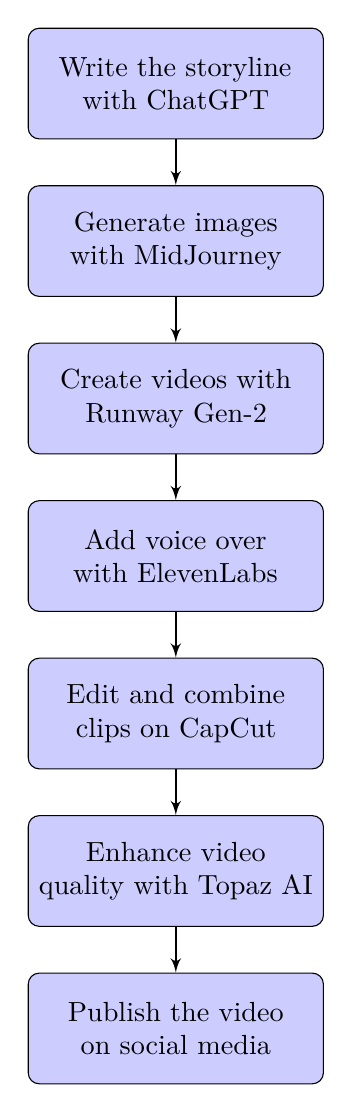
\begin{tikzpicture}[node distance=2cm, auto]
    % Define the style for the nodes
    \tikzstyle{block} = [rectangle, draw, fill=blue!20, text width=10em, text centered, rounded corners, minimum height=4em]
    \tikzstyle{line} = [draw, -latex', thick]
    
    % Place the nodes
    \node [block] (storyline) {Write the storyline with ChatGPT};
    \node [block, below of=storyline] (imagegen) {Generate images with MidJourney};
    \node [block, below of=imagegen] (videogen) {Create videos with Runway Gen-2};
    \node [block, below of=videogen] (voiceover) {Add voice over with ElevenLabs};
    \node [block, below of=voiceover] (videoedit) {Edit and combine clips on CapCut};
    \node [block, below of=videoedit] (videoquality) {Enhance video quality with Topaz AI};
    \node [block, below of=videoquality] (publish) {Publish the video on social media};
    
    % Connect the nodes with paths
    \path [line] (storyline) -- (imagegen);
    \path [line] (imagegen) -- (videogen);
    \path [line] (videogen) -- (voiceover);
    \path [line] (voiceover) -- (videoedit);
    \path [line] (videoedit) -- (videoquality);
    \path [line] (videoquality) -- (publish);
\end{tikzpicture}
\caption{Workflow of the video-creating project}
\end{figure}

\begin{figure}[H]
\centering
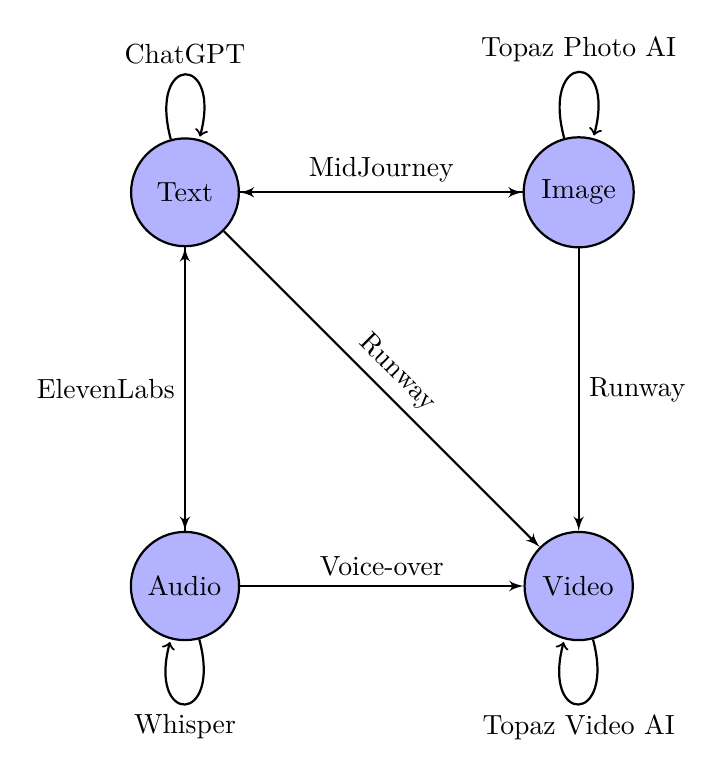
\begin{tikzpicture}[node distance=5cm, auto]
    % Define the style for the nodes
    \tikzstyle{main} = [circle, thick, draw, fill=blue!30, text width=3em, text centered, minimum height=3em]
    \tikzstyle{line} = [draw, -latex', thick]
    
    % Place the nodes
    \node [main] (text) {Text};
    \node [main, right of=text] (image) {Image};
    \node [main, below of=image] (video) {Video};
    \node [main, left of=video] (audio) {Audio};
  
    % Connect the nodes with paths
    \path [line] (text) -- node[above] {MidJourney} (image);
    \path [line] (image) -- (text);
    \path [line] (text) -- (audio);
    \path [line] (text) -- node[sloped, above] {Runway} (video);
    \path [line] (image) -- node[right] {Runway} (video);
    \path [line] (audio) -- node[above] {Voice-over} (video);
    \path [line] (audio) -- node[left] {ElevenLabs} (text);

    \path [line] (text) edge [loop above] node {ChatGPT} (text);
    \path [line] (image) edge [loop above] node {Topaz Photo AI} (image);
    \path [line] (video) edge [loop below] node {Topaz Video AI} (video);
    \path [line] (audio) edge [loop below] node {Whisper} (audio);
  
\end{tikzpicture}
\caption{Relationships in a Multimodal System}
\end{figure}


\section{ChatGPT}
\paragraph{ChatGPT, a state-of-the-art language model developed by OpenAI, operates on the transformer architecture, a breakthrough in deep learning that has revolutionized natural language processing (NLP). It is pre-trained on a diverse corpus of text from the internet, enabling it to grasp a wide array of language nuances, styles, and topics. This pre-training involves unsupervised learning on vast datasets, followed by fine-tuning for specific tasks, which allows ChatGPT to generate coherent, contextually relevant text across many domains without task-specific data. The model's architecture, consisting of multiple layers of transformer blocks, employs self-attention mechanisms to process input text in parallel, significantly improving efficiency and understanding of complex language patterns. Its large parameter count, in the order of billions, captures deep linguistic structures, making it adept at a range of tasks from simple text generation to complex question-answering and summarization without needing explicit programming for each task. The transformer model \cite{vaswani2017attention} and subsequent innovations by OpenAI, including GPT-3's methodology \cite{brown2020language}, underscore the technical foundation and advanced capabilities of ChatGPT, making it a quintessential tool in advancing AI's role in understanding and generating human language.}

\begin{figure}[htbp]
  \centering
  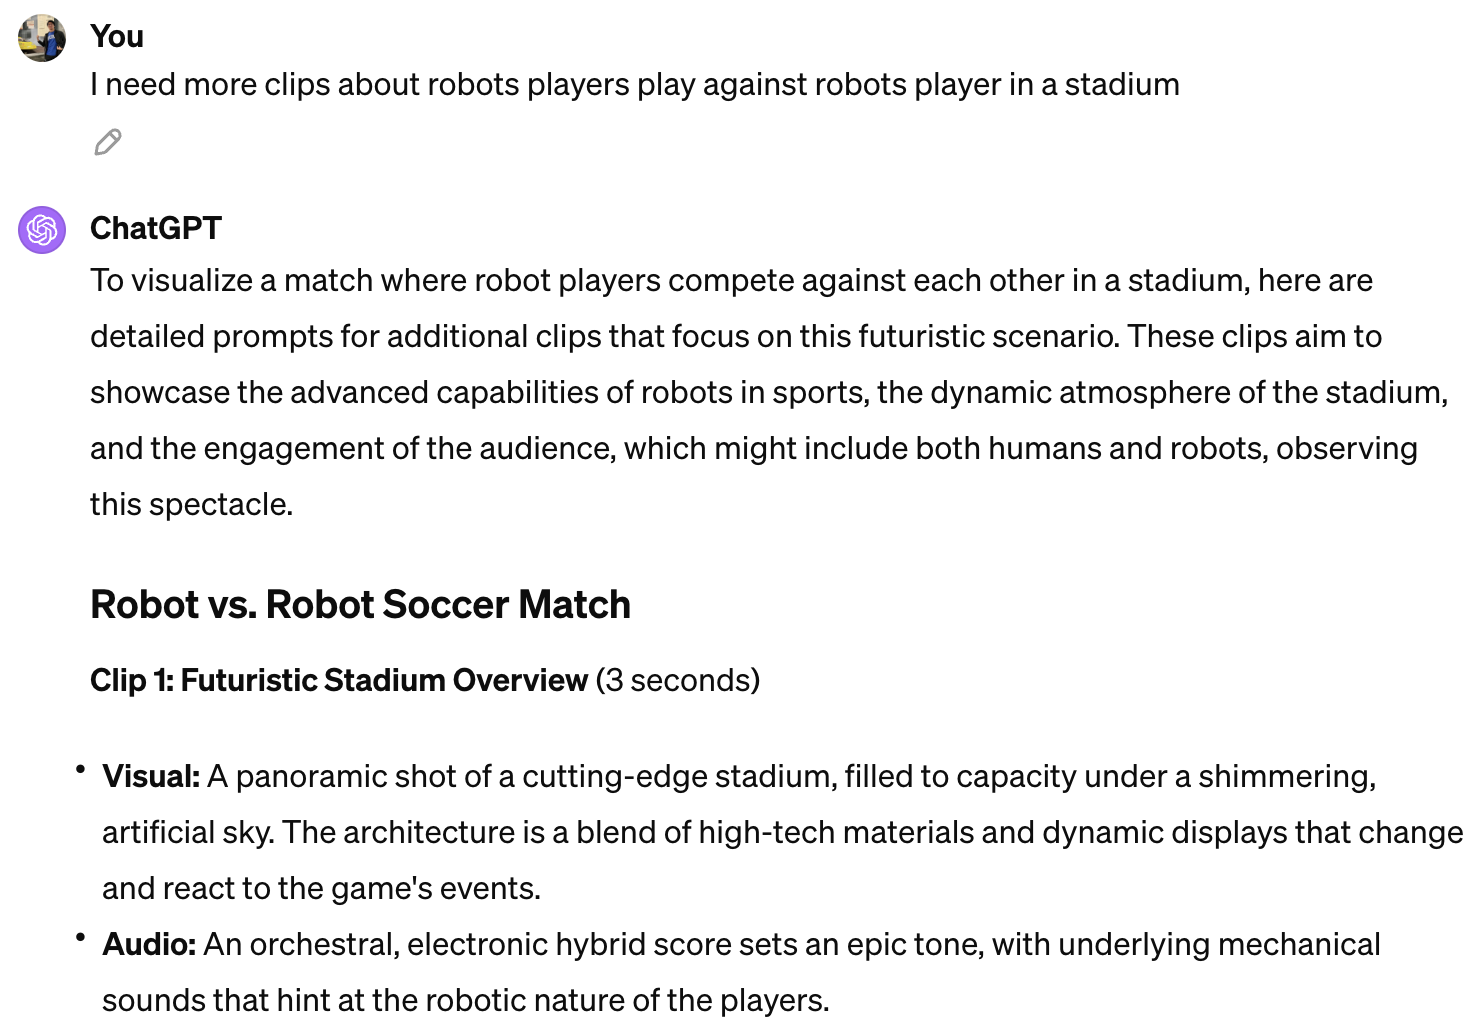
\includegraphics[width=\textwidth]{ChatGPT.png}
  \caption{Using ChatGPT to generate vivid description prompt and prepare for creating the image stills.}
\end{figure}

\section{MidJourney}
\paragraph{MidJourney is an innovative AI model that specializes in generating highly detailed and creative visual content, operating on a complex framework that leverages deep learning techniques to interpret and visualize textual descriptions into compelling images. It utilizes a variant of generative adversarial networks (GANs), where two neural networks work in tandem; one generates images based on textual input, while the other evaluates these images against real-world examples to enhance fidelity and creativity. This iterative process, rooted in the adversarial training methodology, allows MidJourney to produce images that are not only visually stunning but also contextually aligned with the input prompts. The model's architecture is designed to understand and interpret a wide range of descriptive languages, enabling users to guide the creative process through detailed prompts. Advances in GANs and their application in image generation \cite{goodfellow2014generative} \cite{karras2019style}, underpin MidJourney's capabilities. These foundational studies demonstrate the technical and theoretical framework that allows MidJourney to push the boundaries of AI-driven creativity, showcasing its potential to transform visual content generation across various domains.}

\begin{figure}[htbp]
  \centering
  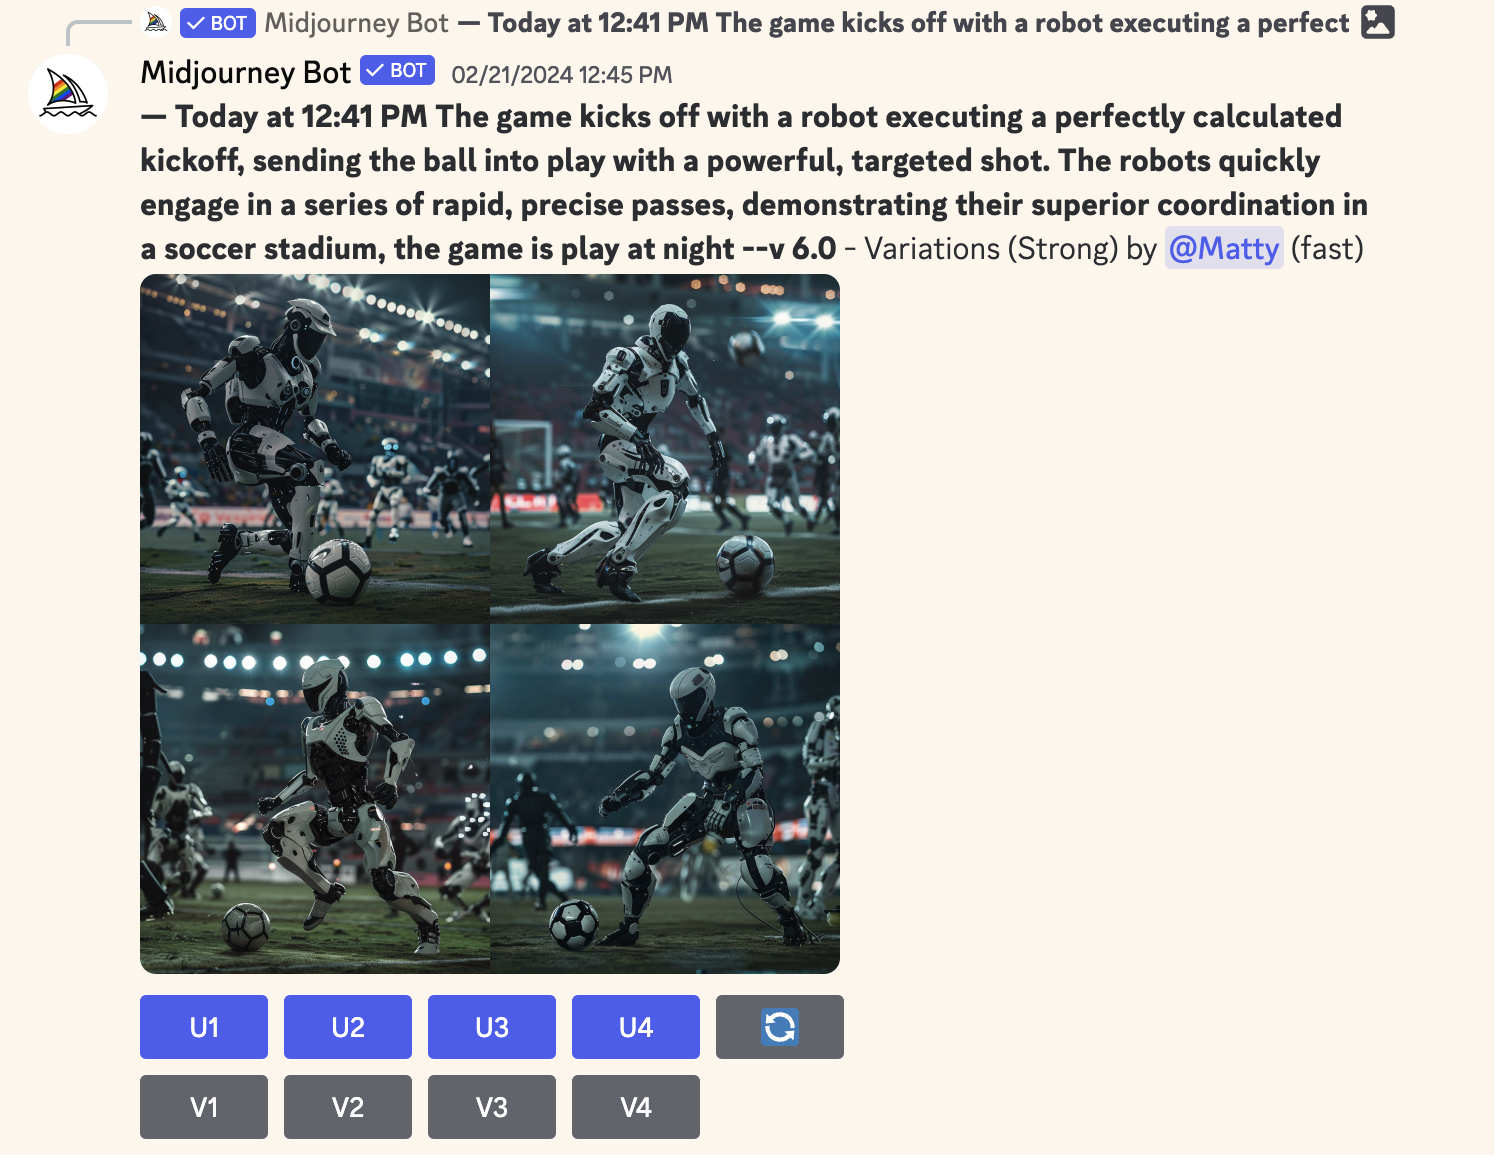
\includegraphics[width=\textwidth]{mj.png}
  \caption{Using ChatGPT's prompts to generate good quality image stills using MidJourney, and then upload them as the key framesto Runway Gen-2 for video clip generation.}
\end{figure}

\section{Runway Gen-2}
\paragraph{Runway Gen-2 is an advanced machine learning platform designed for creative and generative tasks, leveraging cutting-edge models and frameworks to facilitate the creation of digital art, design, and multimedia content. At its core, Runway Gen-2 incorporates a variety of pre-trained models, including those based on GANs (Generative Adversarial Networks) and VAEs (Variational Autoencoders) \cite{kingma2013auto}, allowing users to generate highly detailed and diverse outputs. The platform is built on a modular architecture that supports seamless integration of new models and customizations, making it adaptable to evolving creative needs. It employs a user-friendly interface that democratizes access to complex AI technologies, enabling artists, designers, and creators to experiment with AI without deep technical knowledge. Significant advancements in Runway Gen-2's underlying technology include the optimization of model training and inference processes, which are crucial for real-time performance and high-quality generation capabilities. This optimization is supported by efficient data processing and model deployment strategies, ensuring that users can work with large datasets and complex models effectively.}

\begin{figure}[htbp]
  \centering
  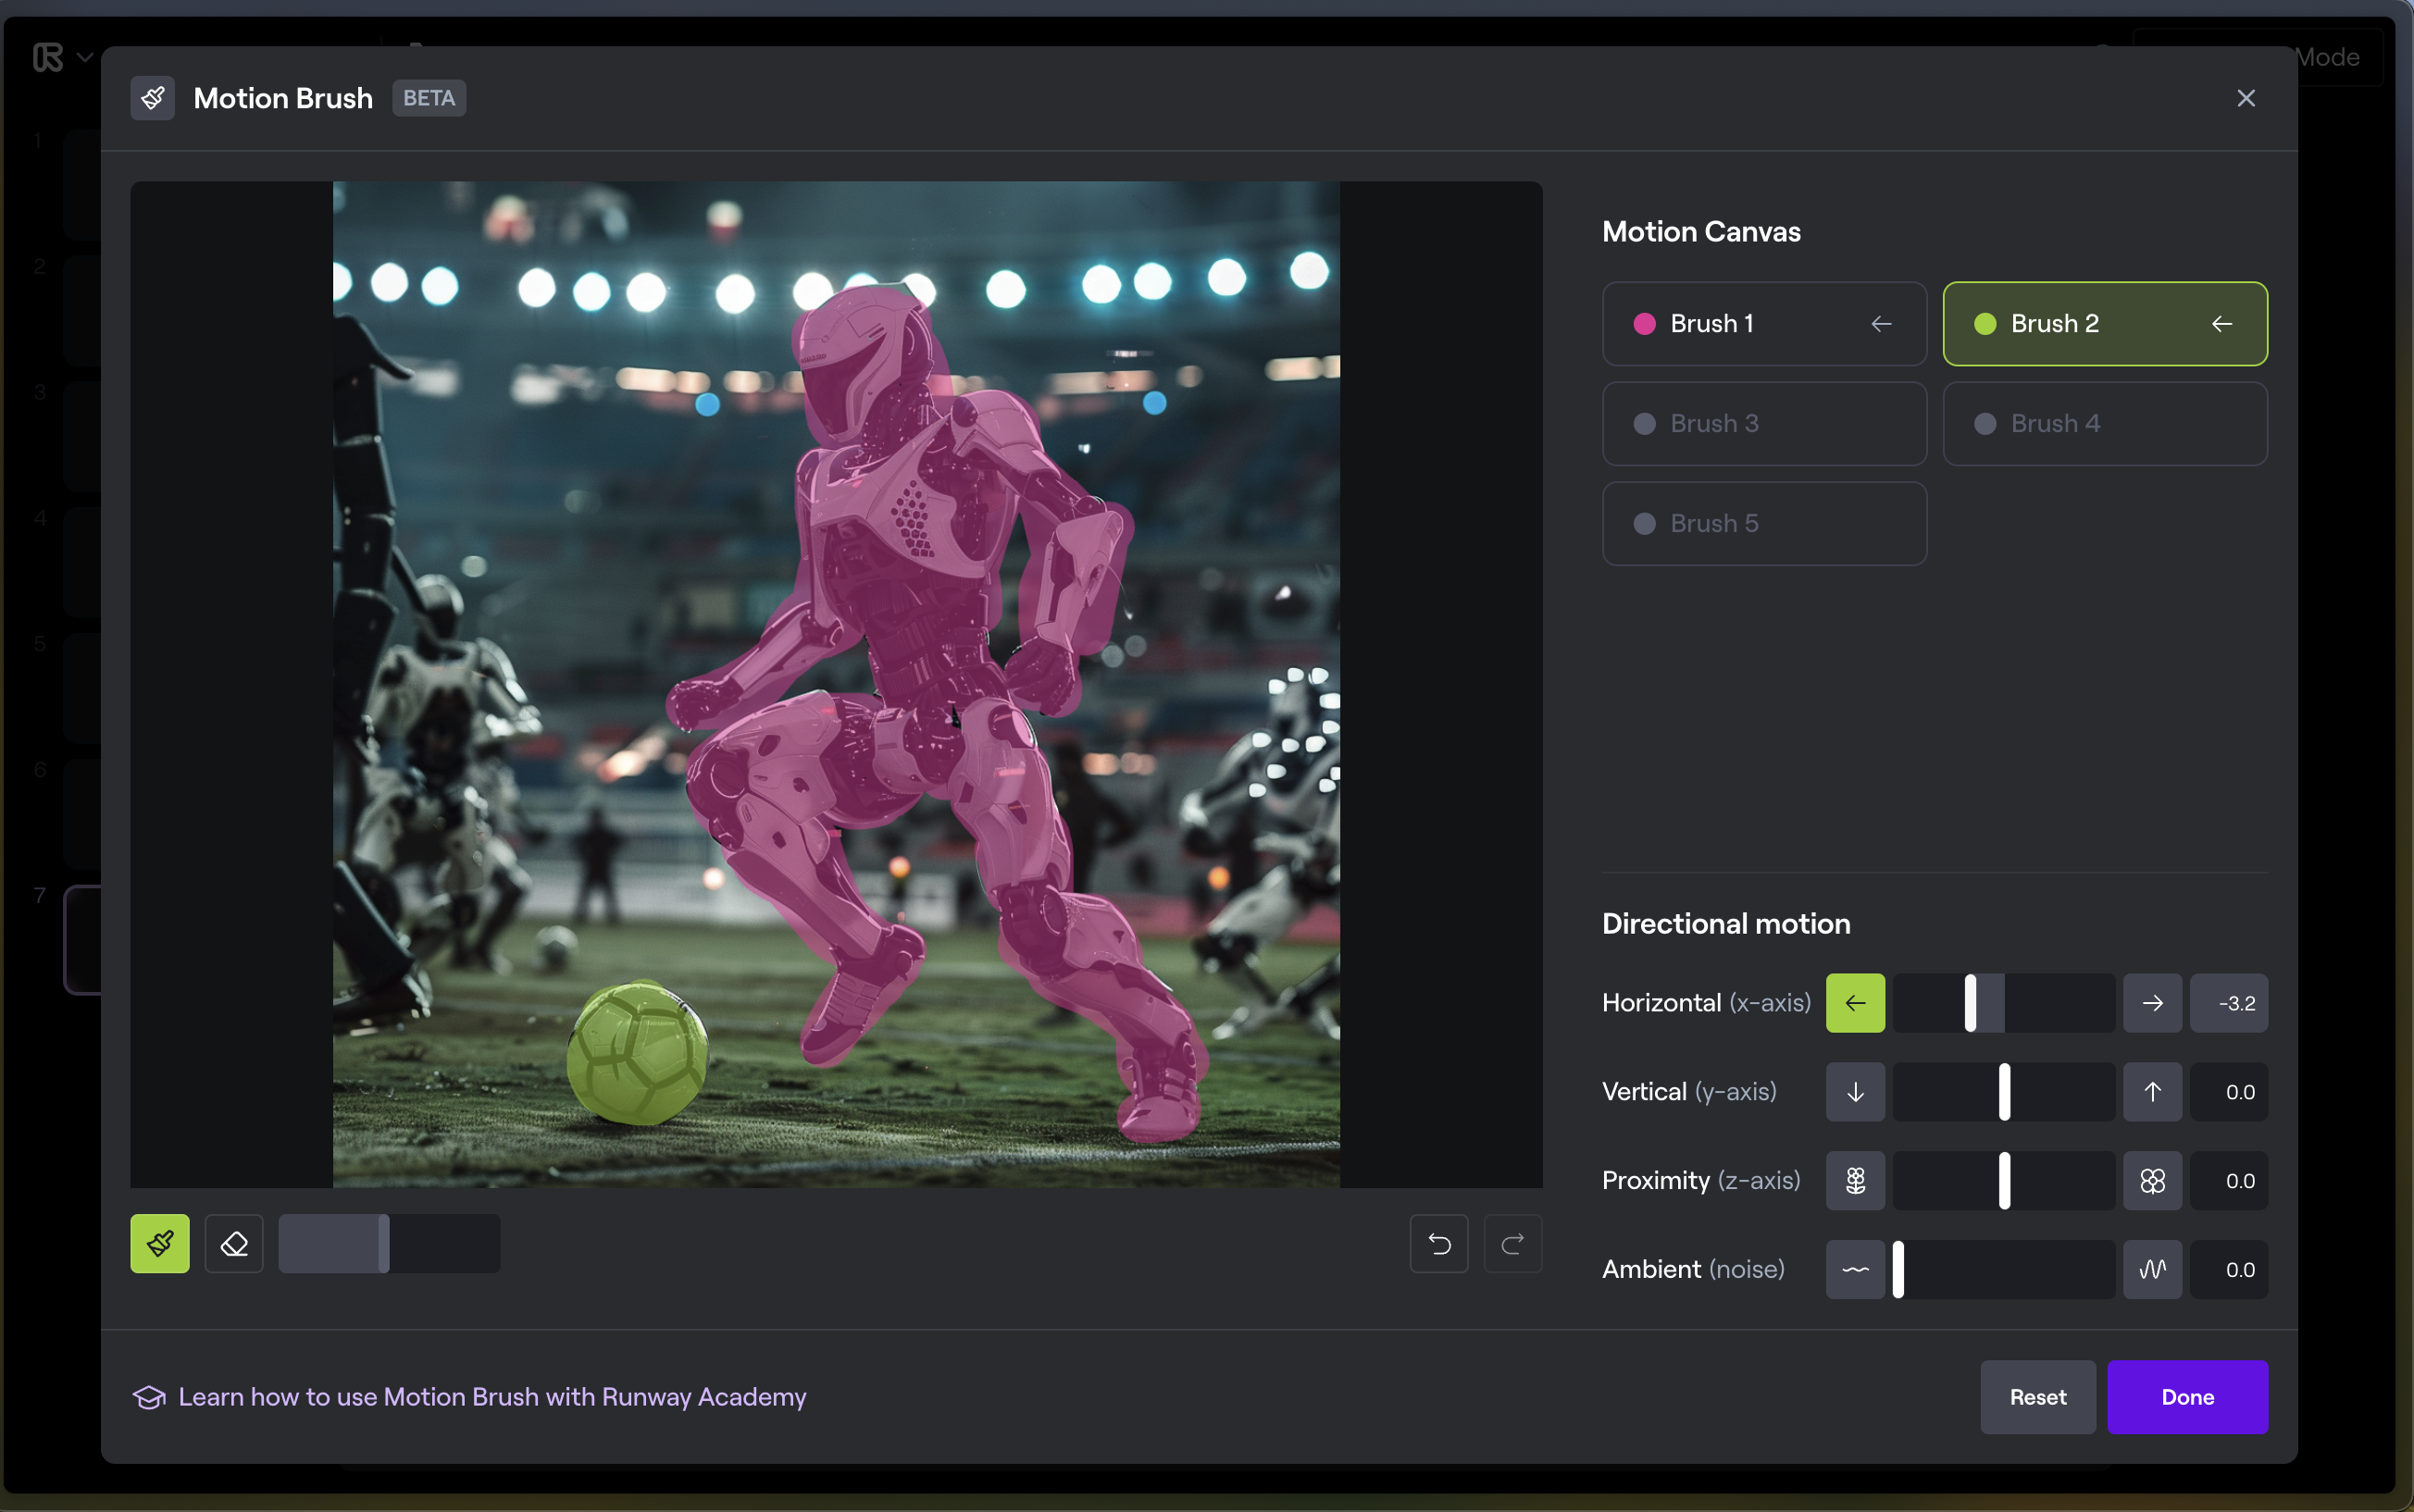
\includegraphics[width=\textwidth]{Runway.png}
  \caption{Using the "Image + Text" mode in Runway Gen-2 to generate the video, with the help of motion brush function to control how the characters move}
\end{figure}


\section{ElevenLabs}
\paragraph{ElevenLabs leverages advanced deep learning techniques to create highly realistic and customizable synthetic voices. At its core, the technology utilizes state-of-the-art voice synthesis models, which are trained on vast datasets of human speech. These models, often based on variants of the transformer neural network architecture, enable the generation of speech that closely mimics human intonation, emotion, and nuances. The process involves two main stages: voice cloning \cite{arik2018neural}, where a target voice is replicated from a small sample, and text-to-speech (TTS) synthesis, where the cloned voice is used to convert written text into spoken words. This sophisticated approach ensures a high degree of vocal fidelity and naturalness, making it suitable for applications in audiobooks, virtual assistants, and more. The methodology behind ElevenLabs' technology draws upon recent advancements in machine learning and NLP, emphasizing the importance of ethical considerations and user consent in voice cloning.}

\begin{figure}[htbp]
  \centering
  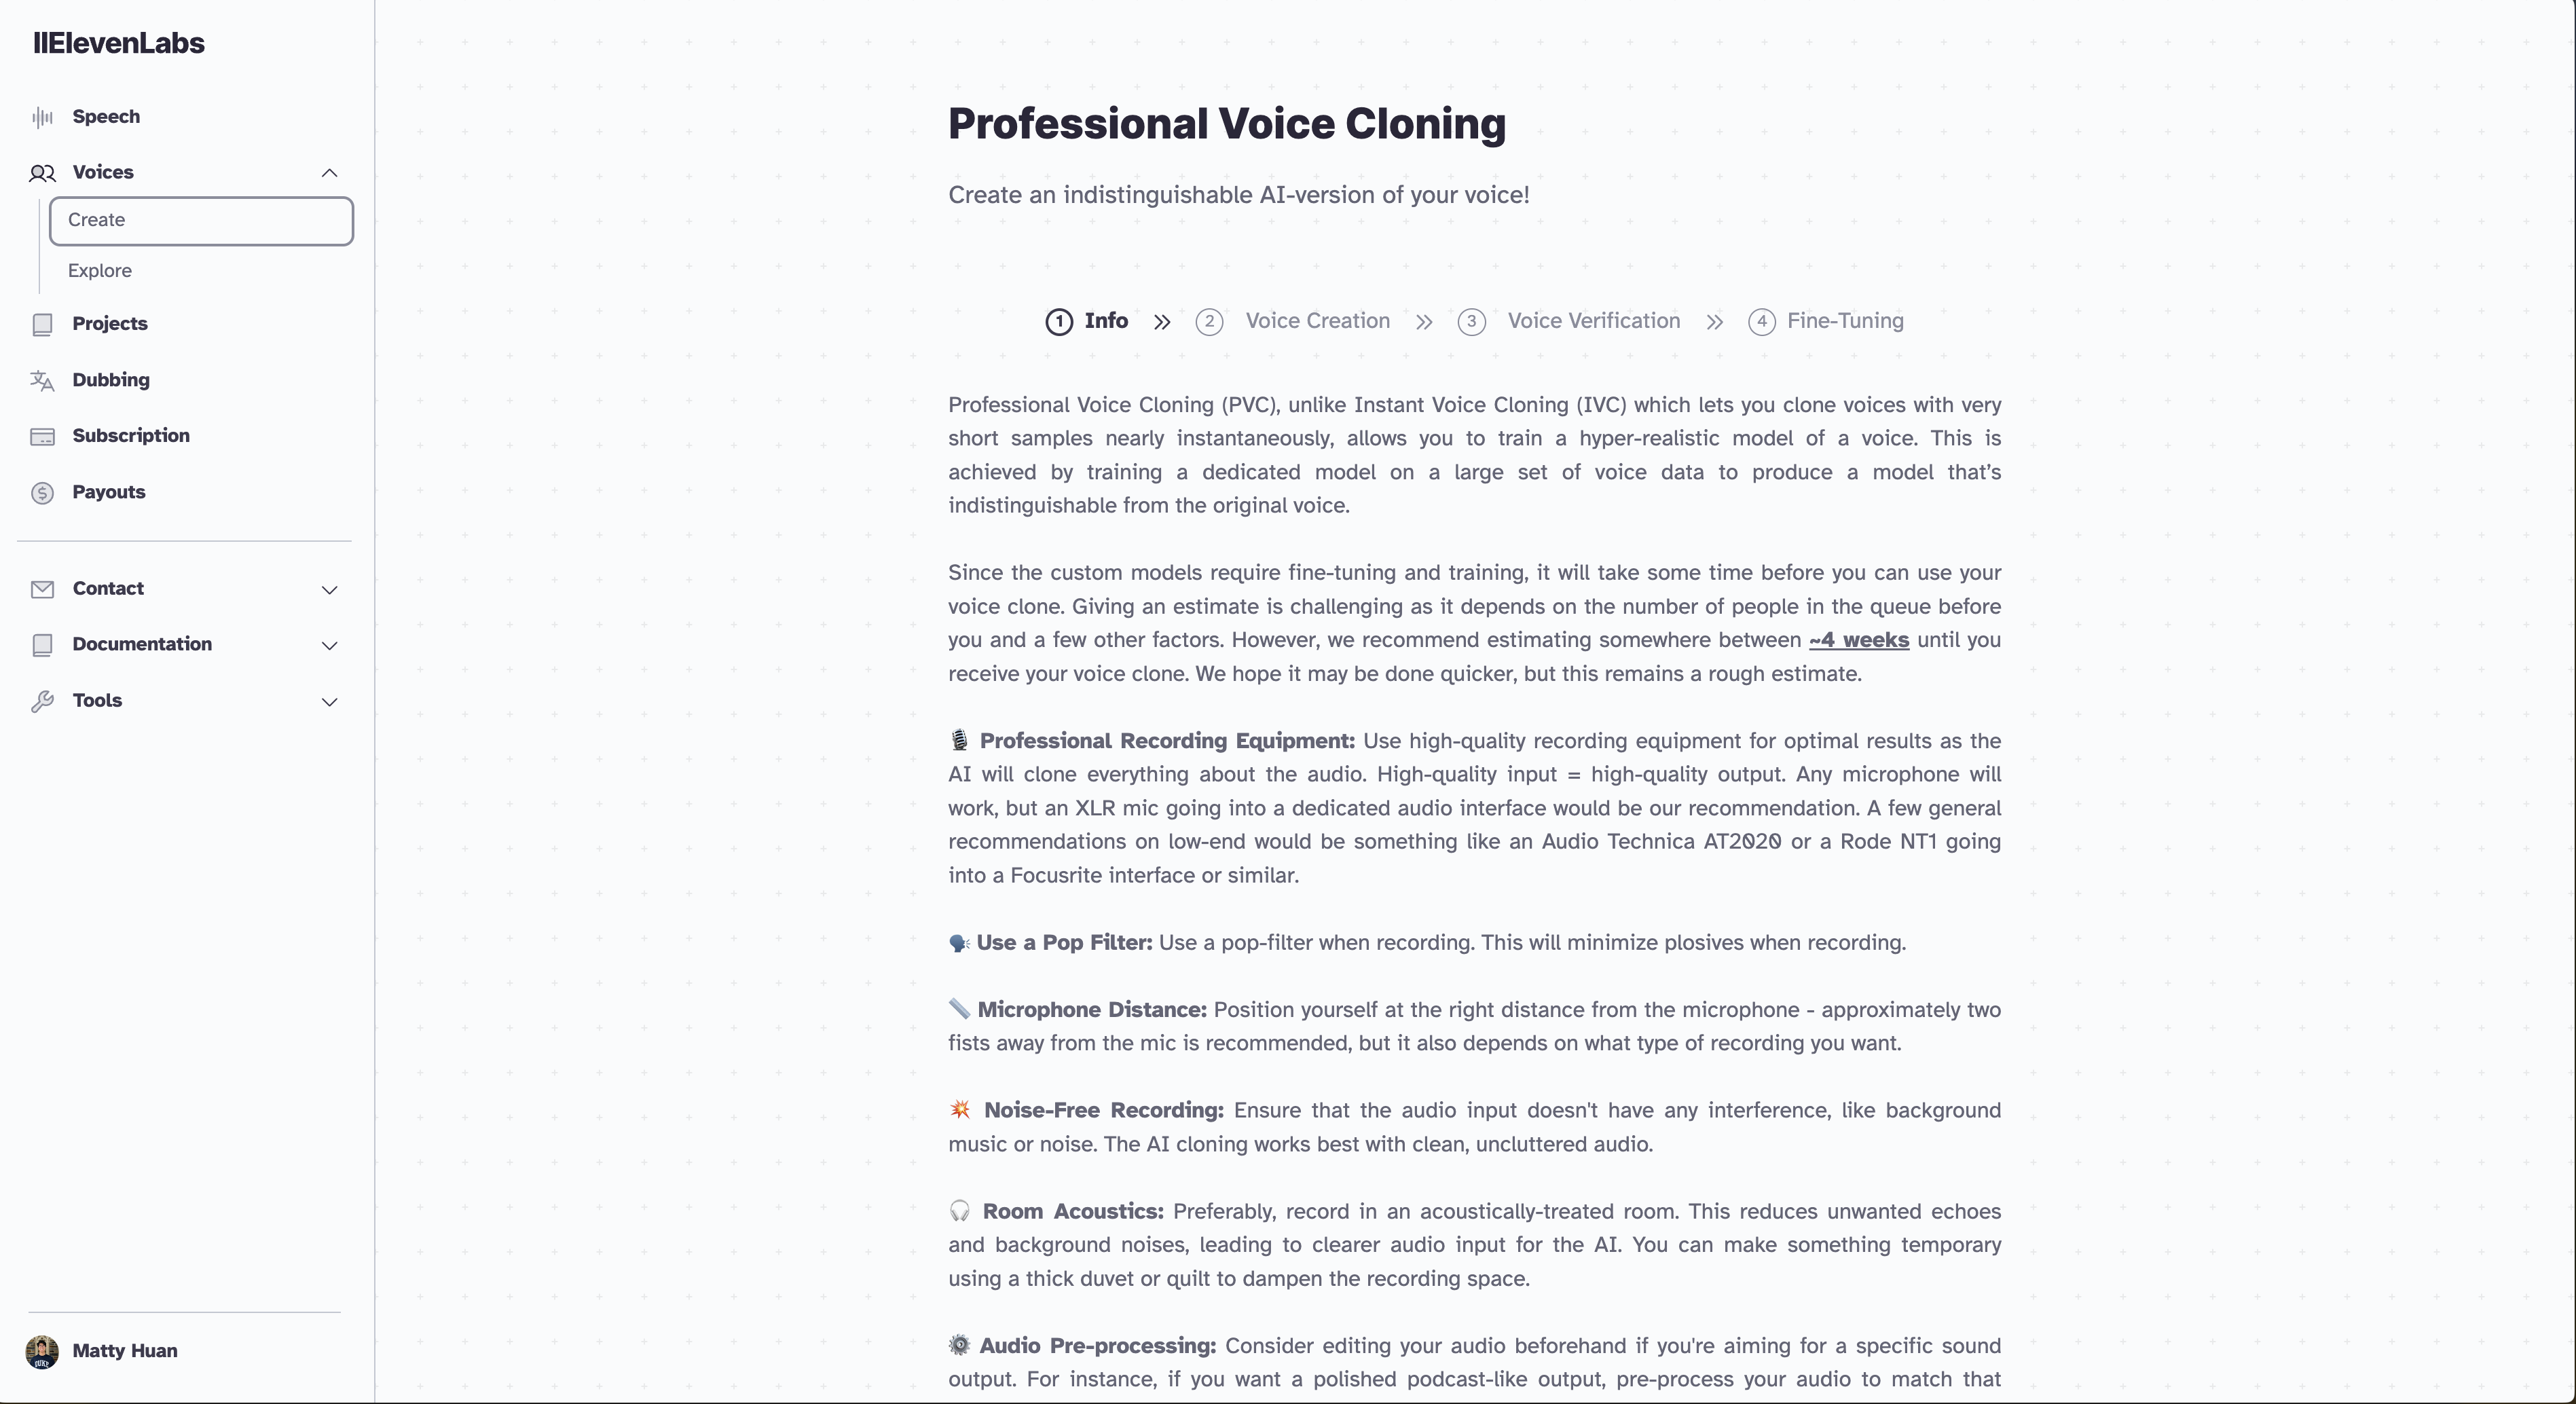
\includegraphics[width=\textwidth]{Voice Cloning.png}
  \caption{Using Professinal Voice Cloning from ElevenLabs to apply text to speech and add the voice over to the video}
\end{figure}

\begin{figure}[htbp]
  \centering
  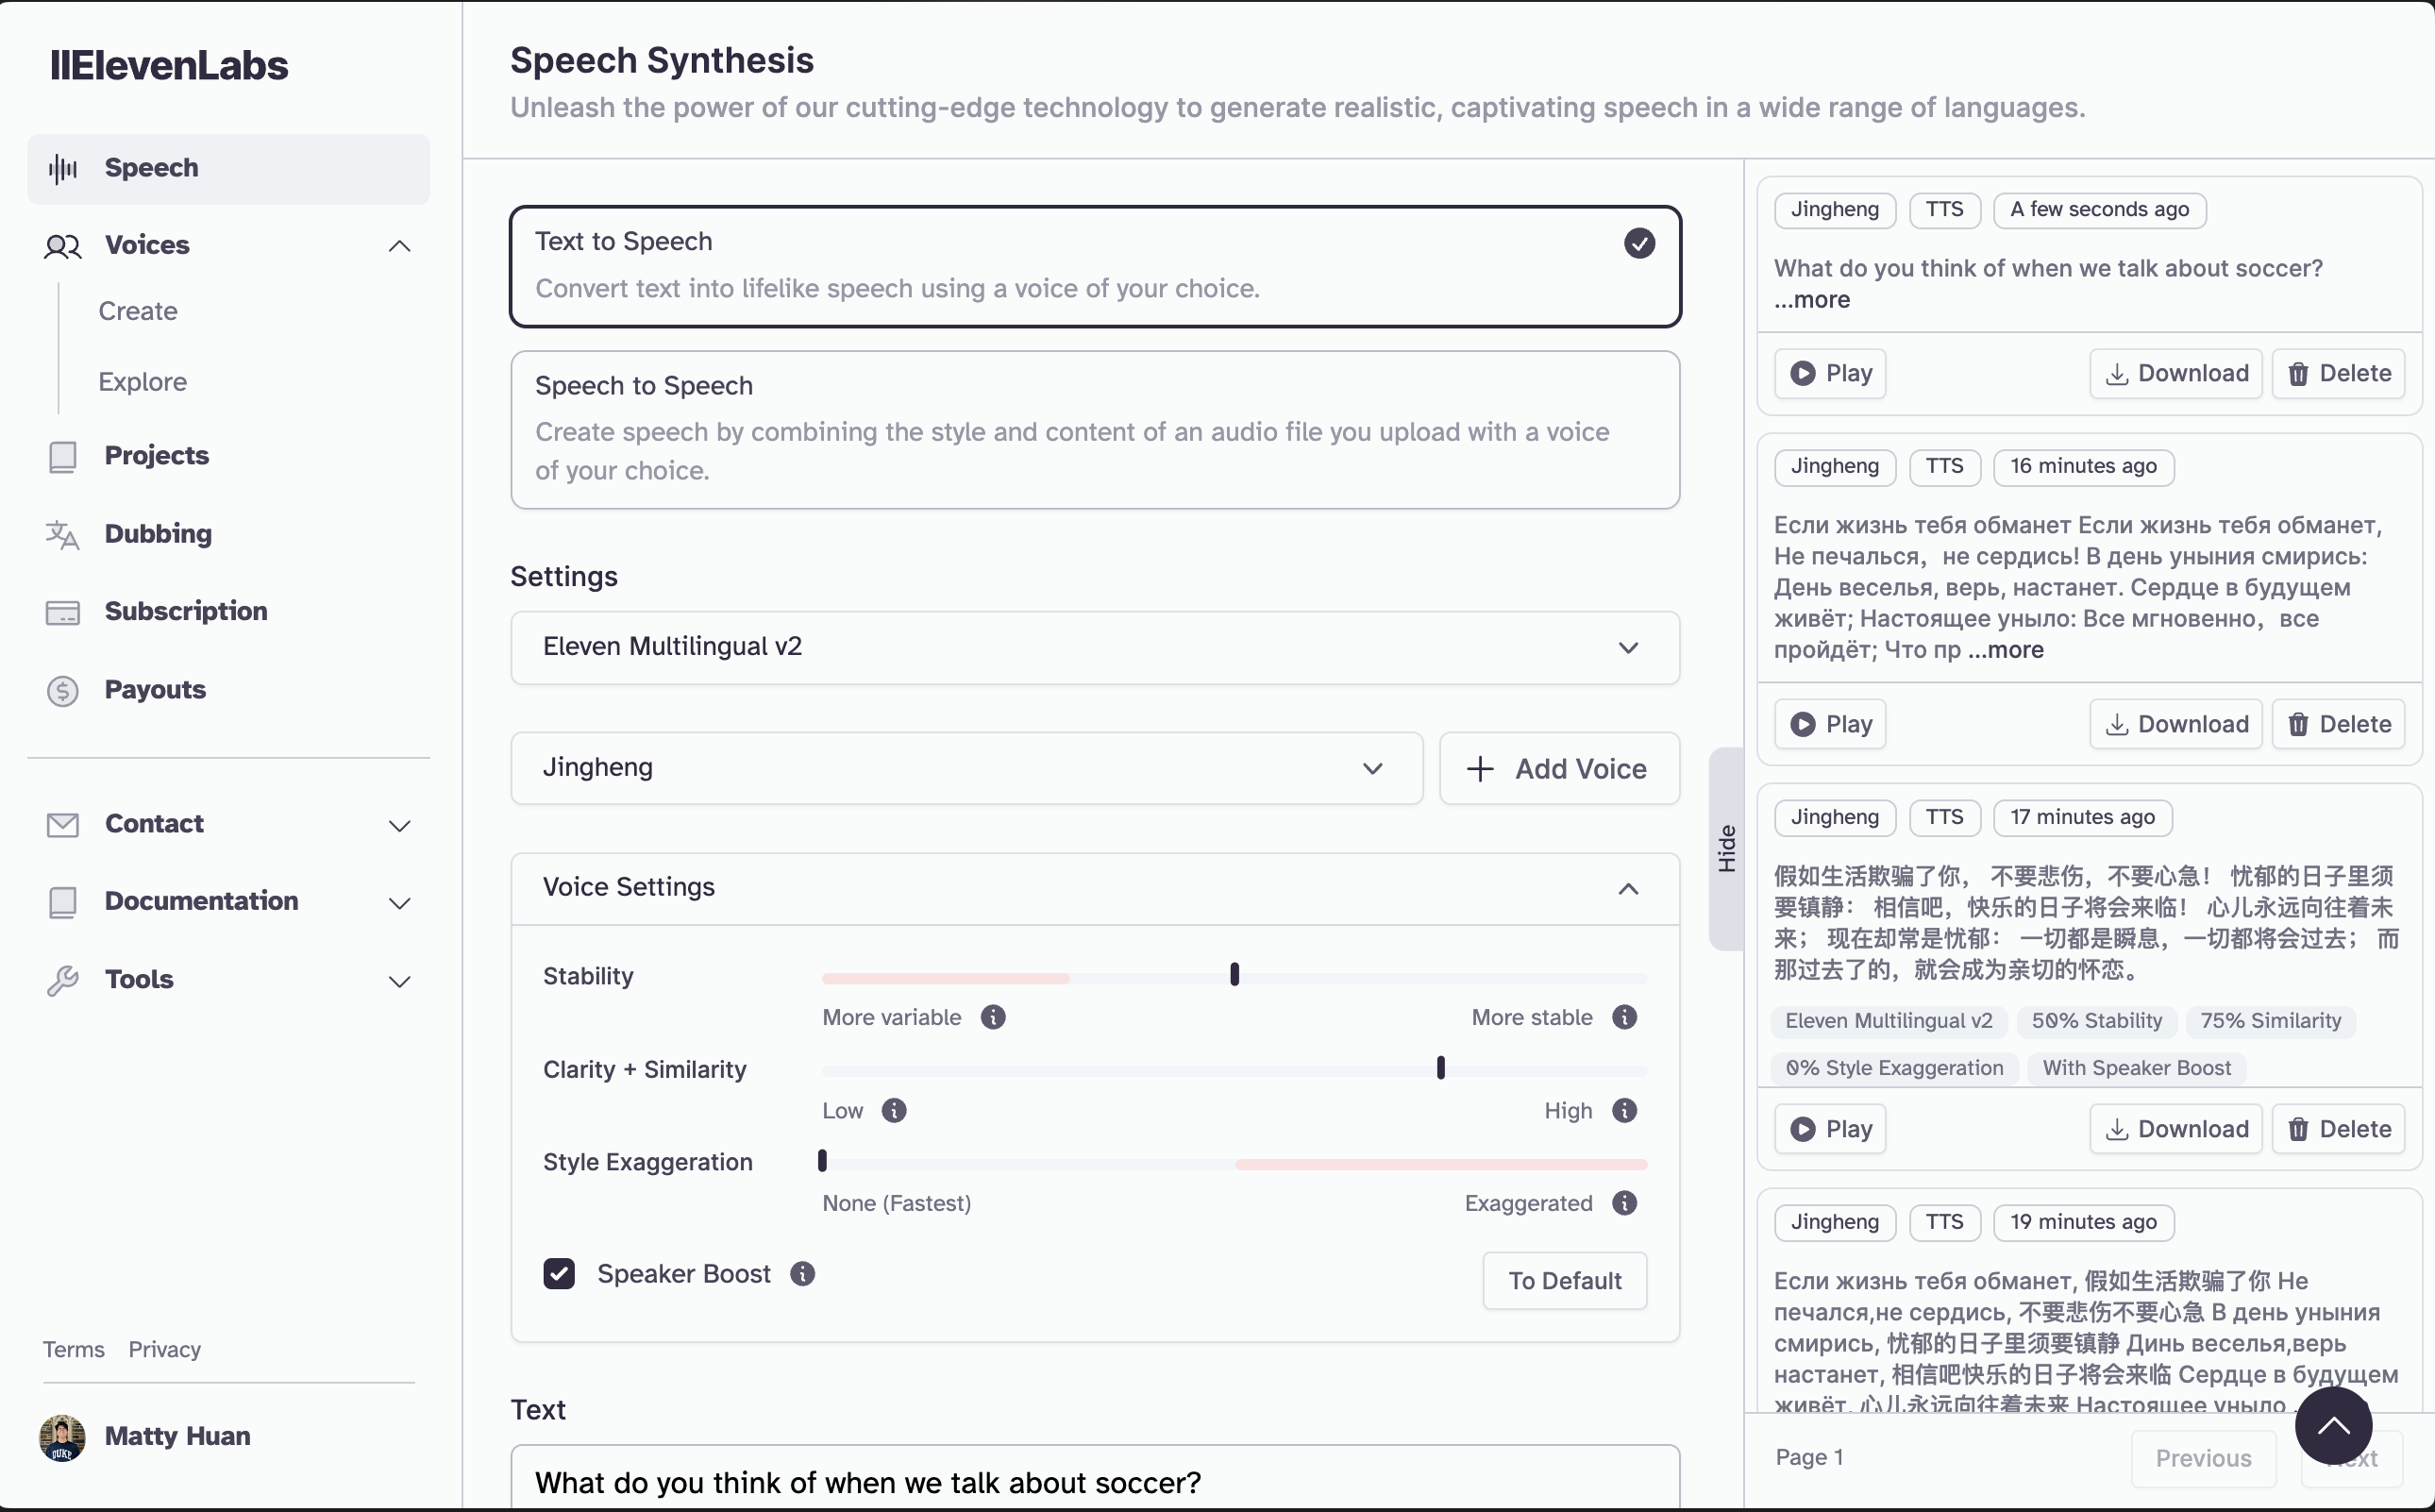
\includegraphics[width=\textwidth]{ElevenLabs.png}
  \caption{Using my clone voice to generate the voice over for the video, I recorded the training set by reading one chapter from the book Elon Musk, the audio file is 14 mins.}
\end{figure}

\section{Topaz AI}
\paragraph{Topaz AI represents a suite of cutting-edge tools designed to enhance image and video quality through deep residual learning \cite{he2016deep}. At its core, Topaz AI utilizes deep learning algorithms to perform tasks such as upscaling, denoising, and sharpening images and videos. The technology is based on convolutional neural networks (CNNs), a type of deep neural network particularly effective for processing visual data. These networks are trained on vast datasets of images, allowing the models to learn how to identify and correct imperfections in new images with remarkable accuracy.}

\begin{figure}[htbp]
  \centering
  \includegraphics[width=\textwidth]{TopazPhoto.png}
  \caption{Using Topaz AI to upscale and improve the video quality, like changing the frame rate from 60 FPS to 120 FPS, removing noise, and sharpen the subject.}
\end{figure}

%%%%%%%%%%%%%%%%%%%%%%%%%%%%%%%%%%%%%%%%%%%%%%%%%%%%%%%%%%%%%%%%%%%%%%%%%%%%%%%%

\chapter{Results \& Discussion}
\label{results}
\section{Overview of Project Outcome}

\paragraph{The video project, a culmination of cutting-edge AI technology and creative vision, presents a narrative that is both visually stunning and thematically profound. Spanning a five-minute duration, it intricately weaves together a series of meticulously crafted scenes, each contributing to a cohesive storyline that explores the symbiotic relationship between humanity and artificial intelligence. Set against the backdrop of futuristic landscapes, the narrative delves into themes of exploration, discovery, and the potential futures shaped by the integration of advanced AI entities within human society. This thematic exploration is brought to life through a variety of scenes, ranging from tranquil, digitally-rendered natural vistas to bustling, urban technoscapes alive with the vibrancy of futuristic life. The selection and progression of scenes are carefully orchestrated to not only captivate the audience with visual splendor but also to provoke thought and reflection on the evolving role of AI in our world.}

\paragraph{The project's success in delivering a compelling narrative is largely attributable to the sophisticated use of AI technologies at each stage of the creative process. From the generation of high-fidelity image stills with MidJourney to the seamless video synthesis facilitated by Runway Gen-2, the tools employed exemplify the potential of AI to transcend traditional boundaries of content creation. The narrative is further enriched with a voiceover, rendered with remarkable realism through ElevenLabs' voice cloning technology, adding a layer of narrative depth that guides the audience through the unfolding story. This integration of AI-driven voice synthesis not only enhances the immersive quality of the video but also demonstrates the nuanced potential of AI in crafting engaging and emotionally resonant storytelling. The video's aesthetic and thematic achievements are underscored by the technical prowess of Topaz AI, which elevates the visual quality through enhancements such as frame rate optimization and noise reduction, ensuring that the final product stands as a testament to the harmony between technological innovation and creative expression.}

\paragraph{This project, through its successful fusion of AI capabilities and creative narrative design, not only showcases the practical applications of these technologies in producing high-quality digital content but also opens a dialogue on the future of storytelling in the age of artificial intelligence. It stands as a compelling example of how AI can be leveraged to create content that is not just visually captivating, but also rich in thematic depth and narrative complexity, challenging us to envision the limitless possibilities of creative expression in the digital era.}

\section{ChatGPT-Assisted Storyline and Description Generation}

\paragraph{In the process of transforming the initial concepts into a coherent and engaging narrative, ChatGPT played an indispensable role, serving as both a creative partner and a critical editor. The tool was pivotal in refining the storyline, ensuring that the flow between scenes was seamless and that the narrative arc was compelling from start to finish. By inputting rough outlines and thematic elements into ChatGPT, the project leveraged the AI's ability to suggest enhancements, fill narrative gaps, and enrich the storyline with deeper context. This collaboration resulted in a narrative that was not only structurally sound but also imbued with a level of depth and nuance that might have been challenging to achieve otherwise. The AI's contributions were particularly valuable in ensuring consistency in tone and pacing, which are crucial for maintaining viewer engagement in a narrative that traverses a range of futuristic landscapes and complex human-AI interactions.}

\paragraph{Beyond the overarching narrative structure, ChatGPT's role extended to the crafting of detailed scene descriptions, which were critical for the subsequent visual content creation phase. For each scene, the AI was provided with a brief, outlining the desired visual elements, mood, and thematic intentions. In response, ChatGPT generated descriptions that vividly captured the essence of these scenes, providing a rich tapestry of details that guided the visual realization process. These descriptions not only included visual cues but also offered suggestions on mood, lighting, and potential dynamics within the scene, thereby ensuring that the visual content was not only aesthetically pleasing but also thematically coherent. The iterative refinement of these descriptions, through a feedback loop between the creators and ChatGPT, exemplified the synergistic potential of combining human creativity with AI's generative capabilities, leading to scene descriptions that were both imaginative and aligned with the project's vision.}

\paragraph{The integration of ChatGPT in this early stage of the project underscores the transformative potential of AI in the realm of creative storytelling and content creation. By harnessing ChatGPT's capabilities, the project not only achieved a higher level of narrative cohesion and detail but also highlighted the broader implications of AI as a tool for creative augmentation. The success of this collaboration between human creativity and artificial intelligence sets a precedent for future projects, suggesting a paradigm where AI's role extends beyond mere assistance to becoming a central component in the creative process. This approach not only enhances the efficiency and depth of content creation but also opens new avenues for exploring complex themes and narratives in digital storytelling.}

\section{Image Stills Generation with MidJourney}

\paragraph{The creation of image stills, a critical component of the video project, was significantly enhanced by the utilization of MidJourney, an AI tool known for its ability to generate visually stunning and highly detailed images. Leveraging the refined scene descriptions developed with the assistance of ChatGPT, MidJourney was tasked with translating these textual narratives into compelling visual art. The process involved feeding the AI with descriptive prompts, meticulously crafted to encapsulate the essence and intricacies of each scene. MidJourney responded with a series of image stills that not only matched the creators' vision in terms of aesthetic appeal but also surpassed expectations by adding layers of complexity and depth to the visual narrative. The images generated by MidJourney stood out for their vivid representation of futuristic concepts, capturing the imagination with their realism and attention to detail. This phase of the project highlighted the AI's ability to interpret and visualize creative prompts, transforming abstract ideas into tangible visual expressions that significantly contributed to the storytelling process.}

\paragraph{The iterative collaboration between the creative team and MidJourney was instrumental in refining the visual output to align closely with the project's thematic goals. Through a process of selection and refinement, the team worked with the AI to fine-tune the images, adjusting elements such as color schemes, composition, and thematic details to ensure coherence with the overall narrative flow. This back-and-forth not only optimized the visual quality of the stills but also ensured that each image contributed effectively to the unfolding story, enhancing the emotional and thematic resonance of the scenes. The flexibility and responsiveness of MidJourney to creative feedback underscored the potential of AI as a dynamic tool in the content creation process, capable of accommodating nuanced artistic direction and contributing creatively to the project's vision.}

\paragraph{The successful integration of AI-generated image stills into the video project underscored the transformative impact of artificial intelligence on the field of digital media production. By leveraging MidJourney's capabilities, the project not only achieved a high degree of visual sophistication but also demonstrated the feasibility of utilizing AI to streamline the content creation process without compromising on creativity or artistic integrity. This approach to visual storytelling, where AI plays a central role in bringing narrative concepts to life, represents a significant advancement in the capabilities of content creators, offering new possibilities for exploring and expressing complex themes through digital media. The collaboration between human creativity and AI in this phase of the project serves as a compelling example of the synergies that can be achieved, paving the way for future endeavors that harness the power of AI to enhance and expand the boundaries of visual art and storytelling.}

\section{Video Clips Generation Using Runway Gen-2}

\paragraph{The transition from static image stills to dynamic video clips marked a pivotal phase in the video project, facilitated by the advanced capabilities of Runway Gen-2. This AI-driven platform, known for its robust video processing and generation features, was tasked with breathing life into the meticulously crafted scenes, transforming the still imagery into seamless and engaging video sequences. Utilizing the "Image + Text" mode, the project team input the detailed scene descriptions and corresponding stills generated by MidJourney into Runway Gen-2. The AI responded by crafting video clips that not only preserved the visual fidelity of the original stills but also introduced motion and continuity, creating a sense of progression and narrative flow. The application of Runway Gen-2's motion brush tool was particularly noteworthy, as it allowed for precise control over the animation of characters and elements within the scenes, ensuring that each movement contributed to the storytelling in a meaningful way. This phase highlighted the AI's ability to interpret creative direction and apply complex video synthesis techniques, thereby enhancing the narrative with dynamic visual storytelling.}

\paragraph{The collaborative process between the creative team and Runway Gen-2 was characterized by an iterative approach, where generated video clips were reviewed and refined to meet the project's exacting standards. Adjustments were made to the pacing, transitions, and animations within the clips, ensuring that each sequence flowed smoothly into the next and that the overall narrative cohesion was maintained. This fine-tuning process underscored the importance of human oversight in achieving the desired outcome, with the creative team leveraging Runway Gen-2's flexibility to enact changes that aligned with the project's vision. The AI's capacity to adapt to creative feedback and generate revised clips efficiently was instrumental in realizing a video that was both visually captivating and narratively compelling. This phase of the project demonstrated the synergistic potential of combining human creativity with AI's technical prowess, achieving a balance between artistic expression and technological innovation.}

\paragraph{The successful integration of AI-generated video clips into the final project underscored the transformative potential of artificial intelligence in the realm of video production. By utilizing Runway Gen-2, the project not only achieved a high level of visual and narrative dynamism but also showcased the feasibility of employing AI to streamline complex video creation processes. This innovative approach to video storytelling, where AI plays a central role in enhancing the visual narrative, represents a forward leap in the digital content creation landscape. It offers content creators new avenues for artistic exploration and expression, enabling the production of rich, immersive narratives that might have been unattainable through traditional methods alone. The collaborative achievements of this phase serve as a testament to the evolving relationship between human creativity and artificial intelligence, highlighting a future where AI's role in creative industries continues to expand, opening up unprecedented possibilities for storytelling and visual communication.}

\section{Voice Over Creation with ElevenLabs}

\paragraph{The addition of a voiceover to the video project represented a critical juncture in enhancing its narrative depth and emotional resonance, achieved through the innovative use of ElevenLabs' voice cloning technology. This phase involved the creation of a synthetic voice that could narrate the video's storyline with a level of expressiveness and nuance akin to a human speaker. By submitting a sample of the desired voice tone and modulation to ElevenLabs, the project team was able to generate a voice clone that not only matched the specified attributes but also conveyed the narrative with an emotional depth that significantly enriched the viewer's experience. This technology's ability to produce a voice that could seamlessly switch between tones—ranging from contemplative to exhilarating—allowed for a dynamic storytelling approach that aligned closely with the video's thematic shifts and narrative pace. The integration of this voiceover into the video project was not just about adding a layer of auditory information; it was about imbuing the narrative with a personal touch that invited the audience into the story, enhancing the engagement and immersion.}

\paragraph{The process of integrating the AI-generated voiceover with the video content underscored the importance of precision in timing and emotional congruence. The project team meticulously aligned the voiceover with the visual sequences, ensuring that each spoken word resonated with the unfolding scenes and actions. This alignment was crucial for maintaining the narrative flow and ensuring that the voiceover amplified, rather than distracted from, the visual storytelling. Adjustments were made to the pacing of the voiceover and the timing of key narrative points to achieve a harmonious balance between the audio and visual elements. The capability of ElevenLabs' technology to fine-tune the voiceover in response to feedback allowed for iterative improvements, resulting in a final product where the voiceover acted as a cohesive and integral component of the storytelling experience.}

\paragraph{The successful incorporation of the voiceover, generated using ElevenLabs' voice cloning technology, into the video project highlights the expanding role of AI in enhancing multimedia content beyond visual elements. This phase of the project illustrates the potential of AI to add depth and emotion to digital storytelling, transforming the way stories are told and experienced. By leveraging such advanced AI tools, content creators can now craft narratives that are more engaging, expressive, and impactful, marking a significant evolution in digital media production. The use of AI-generated voiceovers, in particular, opens up new possibilities for personalizing and enriching content, making it accessible to a broader audience and further blurring the lines between human and machine-generated creativity. This achievement not only exemplifies the technical capabilities of current AI technologies but also points to a future where AI plays a central role in all facets of content creation, offering innovative solutions for storytelling challenges and setting new standards for narrative excellence.}

\section{Video Quality Enhancement with Topaz AI}

\paragraph{The final enhancement phase of the video project, focusing on improving the overall video quality, was adeptly handled using Topaz Video AI. This phase was pivotal in elevating the visual presentation to professional standards, addressing key aspects such as frame rate optimization, noise reduction, and clarity enhancement. Topaz Video AI's advanced deep learning algorithms analyzed the video clips to identify and rectify common issues that affect video quality, such as blurriness, artifacts, and jitter. By converting the frame rate from 60 FPS to 120 FPS, the tool significantly smoothed motion, lending a more fluid and natural feel to the movements within each scene. This adjustment was particularly effective in scenes with fast-paced action or complex animations, where clarity and smoothness are crucial for viewer comprehension and enjoyment.}

\paragraph{Noise reduction was another critical area addressed by Topaz Video AI, which proved essential in maintaining the visual integrity of scenes, especially those generated under less-than-ideal conditions or those requiring a high degree of digital compositing. The AI algorithms worked to selectively remove visual noise without compromising the detail and texture that give each scene its unique character. This delicate balance ensured that the final video maintained a clean and polished look, free from distractions that could detract from the viewer's immersion. Additionally, the tool's ability to enhance the overall sharpness and clarity of the video content helped in accentuating details that might otherwise go unnoticed, making each frame more impactful and engaging.}

\paragraph{The integration of Topaz Video AI into the project's workflow underscores the transformative impact of AI on video production, particularly in the post-production phase. By leveraging the tool's capabilities, the project achieved a level of visual quality that rivals professional production standards, showcasing the potential of AI to streamline and enhance the content creation process. This phase not only highlighted the technical proficiency of current AI tools in improving video aesthetics but also demonstrated the practical value of AI in resolving common challenges faced by content creators. The improvements made through Topaz Video AI brought the project to its culmination, with a final product that stood as a testament to the synergy between human creativity and artificial intelligence. This accomplishment illustrates the evolving landscape of digital media production, where AI technologies play an increasingly central role in enabling creators to achieve their vision with greater efficiency and precision, pushing the boundaries of what is possible in storytelling and visual communication.}

%%%%%%%%%%%%%%%%%%%%%%%%%%%%%%%%%%%%%%%%%%%%%%%%%%%%%%%%%%%%%%%%%%%%%%%%%%%%%%%%

\paragraph{The roadmap for future development in AI's application to image, video, and now sound generation encapsulates a journey from foundational models to the cusp of groundbreaking innovations, illustrating a trajectory that is as diverse as it is profound. This progression can be dissected into several key stages, each marking significant milestones in the evolution of AI technologies and their applications.}

\section{Foundational Models}
\paragraph{The journey into the realms of Artificial Intelligence (AI) commenced with the development of basic machine learning algorithms and the advent of neural networks, marking a seminal phase in the evolution of computational intelligence. These initial models established a fundamental framework for the analysis and interpretation of data patterns, heralding the dawn of computational learning. By enabling machines to learn from and make predictions based on data, these foundational technologies set the stage for a radical transformation in the way that information is processed and utilized. Neural networks, in particular, with their ability to mimic the neural structures of the human brain, introduced a novel paradigm for machine learning, facilitating the development of systems capable of performing complex tasks such as image recognition, natural language processing, and decision making with unprecedented accuracy. This era of AI research and development, characterized by the exploration and refinement of machine learning algorithms and neural network architectures, laid the crucial groundwork for subsequent advancements in AI, propelling the field towards the sophisticated and versatile AI systems we see today \cite{huang2022large}. The significance of these early models cannot be overstated, as they not only provided the initial impetus for AI research but also continue to underpin the ongoing exploration and expansion of AI capabilities across various domains.}

\section{Specialized Architectures}
\paragraph{The introduction of specialized architectures, notably Generative Adversarial Networks (GANs) and Diffusion Models, represents a watershed moment in the advancement of Artificial Intelligence (AI), heralding a new era of sophistication in AI capabilities. GANs, conceptualized as a system of two neural networks contesting with each other in a generative adversarial process, have fundamentally transformed the landscape of synthetic media creation. This architecture's unique capability to produce high-fidelity images and videos has significantly elevated the standard of realism and detail attainable in digital content, marking a departure from previous limitations. Similarly, Diffusion Models, which iteratively refine random noise into structured images through a reverse Markov process, have further extended the possibilities for generating intricate and lifelike synthetic visuals. These developments have not only expanded the horizons of what is achievable with AI in the realm of digital media but have also laid the foundation for novel applications across diverse fields such as entertainment, healthcare, and education. The impact of these specialized architectures on the AI domain has been profound, catalyzing a shift towards the creation of more realistic, dynamic, and nuanced digital experiences, and setting new benchmarks for the quality of AI-generated content \cite{granot2022drop}. The advent of GANs and Diffusion Models thus marks a significant milestone in the evolution of AI, underscoring the technology's growing ability to mimic, and in some cases surpass, the intricacies of human perception and creativity.}

\section{Ethical and Societal Considerations}
\paragraph{As Artificial Intelligence (AI) technologies have evolved and matured, there has been a discernible shift towards addressing the broader ethical and societal implications associated with AI-generated content. This phase of AI development is characterized by a heightened awareness of the potential for biases embedded within AI systems, leading to concerted efforts aimed at identifying, understanding, and mitigating these biases to ensure fairness and equity in AI applications. Additionally, the capacity of AI to generate highly realistic synthetic media, such as deepfakes, has raised significant concerns about the potential for misuse in spreading misinformation and manipulating public perception. In response, researchers and developers are increasingly prioritizing the development of AI technologies that incorporate ethical considerations from the outset, emphasizing the creation of systems that are not only technologically advanced but also socially responsible. This involves the implementation of robust mechanisms for the detection and prevention of AI-generated content that could be used for malicious purposes, alongside initiatives to promote transparency and accountability in AI development processes. The focus on ethical and societal considerations marks a critical evolution in the field of AI, reflecting a growing recognition of the technology's profound impact on society and the imperative to guide its development in a direction that maximizes benefits while minimizing harms. This shift towards ethically conscious AI development is fundamental to ensuring that the advancements in AI technology contribute positively to society, fostering an environment where innovation is balanced with responsibility \cite{esposito2023mitigating}.}

\section{Efficiency and Scalability}
\paragraph{The current focus within the field of Artificial Intelligence (AI) on enhancing efficiency and scalability underscores a pivotal shift towards developing algorithms that are both robust and adaptable to the exigencies of real-time and large-scale applications. This trend is driven by the increasing demand for AI technologies that can process and analyze vast amounts of data swiftly and accurately, facilitating their integration into various aspects of digital media production, from content creation to distribution. Innovations aimed at optimizing processing speeds are critical in this context, as they enable AI systems to perform complex computations more rapidly, thereby reducing latency and improving the user experience. Similarly, efforts to augment the scalability of AI systems are essential for accommodating the exponential growth in data volumes and the complexity of tasks that AI is expected to handle. These advancements are not merely technical achievements but also reflect a broader imperative to ensure that AI technologies remain relevant and effective in a rapidly evolving digital landscape. By prioritizing efficiency and scalability, researchers and developers are working to create AI systems that are not only theoretically advanced but also practically applicable, capable of supporting the dynamic and diverse needs of modern digital media production \cite{habibian2021skip}. This alignment of AI development with the practical demands of real-world applications is crucial for the continued integration and expansion of AI across different sectors, promising to unlock new possibilities for innovation and creativity in the digital age.}

\section{Extension to Sound Generation}
\paragraph{In tandem with the significant strides made in image and video synthesis, the exploration of Artificial Intelligence (AI) within the realm of sound generation has marked a pivotal expansion of AI's capabilities, catalyzing a transformative shift in the creation and manipulation of audio content. Advancements in AI-driven music composition, voice synthesis, and sound effects generation are at the forefront of this evolution, employing sophisticated algorithms to produce audio that is not only more natural and lifelike but also dynamic and sensitive to context. These developments in sound generation are predicated on deep learning models that analyze and learn from vast datasets of existing audio, enabling the generation of sound that can adapt to varying narrative and environmental cues, thereby enriching the auditory experience across a wide range of applications, from interactive media to immersive virtual environments. The integration of AI in sound generation thus represents a significant milestone, highlighting the technology's capacity to extend its influence beyond the visual domain and into the broader spectrum of multimedia content creation. This holistic approach to AI application in multimedia not only enhances the realism and engagement of digital experiences but also underscores the technology's role in shaping the future of content creation, where AI's contribution is envisaged to permeate all aspects of digital media, offering unprecedented opportunities for innovation and creativity.}

\section{Future Directions}
\paragraph{Looking ahead, the trajectory of Artificial Intelligence (AI) development is increasingly oriented towards the integration and unification of diverse AI methodologies to forge comprehensive and holistic solutions, a direction that promises to significantly broaden the scope and impact of AI applications. This forward-thinking approach aims not only to enhance existing capabilities in image and video synthesis but also to extend AI's prowess into the realms of 3D object generation and the simulation of functional machines, thereby pushing the boundaries of digital creation into new dimensions. Moreover, the exploration of advanced applications in sound generation by leveraging AI techniques is set to further dissolve the distinctions between AI-generated content and the tangible reality, offering experiences that are more immersive and indistinguishable from the natural world. Such unified AI systems, which amalgamate various techniques ranging from Generative Adversarial Networks (GANs) and Diffusion Models to Neural Cellular Automata, are poised to transform a wide array of fields including entertainment, education, healthcare, and manufacturing. By enabling the creation of dynamic, interactive, and highly realistic digital environments and objects, this integrative approach underscores the potential of AI to not just augment but fundamentally redefine the landscape of digital content creation. The envisioned future of AI, as a confluence of disparate techniques yielding seamlessly integrated solutions, heralds a new era of innovation where the lines between digital and physical realities are increasingly blurred, fostering unprecedented levels of creativity and interaction \cite{esser2022towards}.}

%%%%%%%%%%%%%%%%%%%%%%%%%%%%%%%%%%%%%%%%%%%%%%%%%%%%%%%%%%%%%%%%%%%%%%%%%%%%%%%%

\chapter{Conclusions}
\label{conclusions}

\paragraph{This comprehensive study has elucidated the transformative role of Artificial Intelligence (AI) in the domains of image, video, and sound generation, underscoring the profound implications these technologies hold for the future of digital media production. Through a meticulous exploration of Generative Adversarial Networks (GANs), Diffusion Models, and Neural Cellular Automata, the research has unveiled the significant advancements in AI-driven generative technologies, demonstrating their capacity to produce outputs that are not only photorealistic but also creatively unparalleled. The application of these AI models across various sectors, from healthcare and entertainment to education and digital manufacturing, signifies a paradigm shift in how content is conceived, created, and consumed. The integration of AI in these processes not only enhances efficiency and scalability but also opens up new vistas for innovation, allowing for the creation of content that transcends traditional boundaries of creativity and realism. Furthermore, the critical assessment of the ethical landscape surrounding AI-generated content has highlighted the importance of developing robust ethical guidelines and frameworks to govern the use of these powerful technologies, ensuring that they contribute positively to society and do not perpetuate existing biases or facilitate misinformation.}

\paragraph{The project's successful utilization of AI technologies like ChatGPT, MidJourney, Runway Gen-2, ElevenLabs, and Topaz Video AI in creating a compelling video narrative serves as a tangible testament to the potential of AI to revolutionize content creation. The synergy between AI-generated text, images, videos, and voiceovers has not only achieved a high degree of narrative cohesion and visual sophistication but also showcased the practical feasibility of employing AI in streamlining complex production processes without sacrificing artistic integrity. This harmonious integration of AI with human creativity has paved the way for a new era of storytelling, where digital narratives are more engaging, expressive, and immersive. The project's outcomes emphasize the importance of a collaborative approach to AI-driven content creation, where human oversight and creative input guide the AI's capabilities towards achieving a shared vision, thus maximizing the potential of these technologies to enhance storytelling and visual communication.}

\paragraph{Looking forward, the trajectory of AI in digital media production is set towards further integration and unification of diverse AI methodologies, promising to expand the scope and impact of AI applications across all facets of content creation. The continuous evolution of AI technologies is poised to redefine the landscape of digital content creation, blurring the lines between digital and physical realities and fostering new levels of creativity and interaction. As AI systems become more autonomous and creative, the imperative for ethical considerations and guidelines becomes increasingly paramount, ensuring that the advancements in AI not only push the boundaries of what is possible in content creation but also align with societal values and ethical principles. The future of AI in digital media production is bright, heralding a new chapter in creative expression and storytelling that is bound only by the limits of our imagination. This study not only contributes to the academic discourse on AI and generative media but also provides a roadmap for future explorations in this dynamic and evolving field.}
%%%%%%%%%%%%%%%%%%%%%%%%%%%%%%%%%%%%%%%%%%%%%%%%%%%%%%%%%%%%%%%%%%%%%%%%%%%%%%%%

\chapter*{References}
\label{references}
\addcontentsline{toc}{chapter}{References}



\printbibliography[heading=none]


%%%%%%%%%%%%%%%%%%%%%%%%%%%%%%%%%%%%%%%%%%%%%%%%%%%%%%%%%%%%%%%%%%%%%%%%%%%%%%%%

\appendix

\chapter{Additional Material}
\label{appendix-a}

The link of the video is here: \url{https://youtube.com/shorts/C_Ng1JBiA-c?feature=shared}

\end{document}